%%%%%%%%%%%%%%%%%%%%%%%%%%%%%%%%%%%%%%%%%
% This document provides a sample senior
% thesis proposal template for use
% by Allegheny's Computer Science majors.
%
% This template was adopted from Jeremie Gillet
% Ref: https://github.com/oist/LaTeX-templates
%
% Author: Janyl Jumadinova
% Last Updated: November 5, 2019
%
%%%%%%%%%%%%%%%%%%%%%%%%%%%%%%%%%%%%%%%%%

%----------------------------------------------------------------------------------------
%	PACKAGES AND OTHER DOCUMENT CONFIGURATIONS
%----------------------------------------------------------------------------------------

\documentclass[12pt,oneside]{book} % 12 pt font, one-sided book style
\usepackage[a4paper, includehead, headheight=0.6cm, inner=3cm ,outer=2.5cm, top=2.5 cm, bottom=2.5cm]{geometry}  % Changing size of document
\usepackage[english]{babel} % The document is in English
\usepackage[utf8]{inputenc} % UTF8 encoding
\usepackage[T1]{fontenc} % Font encoding

\usepackage{graphicx} % For including images
\graphicspath{{./images/}} % Specifies the directory where images are stored

\usepackage{longtable} % tables that can span several pages
\usepackage[bf]{caption} % caption: FIG in bold
\usepackage{fancyhdr} % For the headers

\newcommand{\numberedchapter}{ % Preparation for numbered chapters
	\cleardoublepage % To make sure the previous headers are passed
	\fancyhead[RE]{{\bfseries \leftmark}}% Headers for left pages
	\fancyhead[LO]{{\bfseries \rightmark}}}% Headers for right pages
\newcommand{\unnumberedchapter}[1]{ % Preparation for unnumbered chapters
	\cleardoublepage % To make sure the previous headers are passed
	\addcontentsline{toc}{chapter}{#1} % Also adds the chapter name to the Contents
	\fancyhead[RE]{{\bfseries #1}} % Headers for left pages
	\fancyhead[LO]{}}%Headers for right pages

\usepackage{emptypage} % No headers on an empty page

% Tikz
\usepackage{tikz}

% Code snippet package
\usepackage{listings}

% Directory diagram package
\usepackage{dirtree}

% Algorithms
\usepackage[linesnumbered,ruled,vlined]{algorithm2e}

\usepackage{eso-pic} % For the background picture on the title page
\newcommand\BackgroundPic{%
\put(0,-120){%
\parbox[b][\paperheight]{\paperwidth}{%
\vfill
\centering

\includegraphics[width=4in]{images/logo}%
\vfill
}}}

\usepackage{hyperref} % Adds clickable links at references

%----------------------------------------------------------------------------------------
%	ADD YOUR CUSTOM VALUES, COMMANDS AND PACKAGES
%----------------------------------------------------------------------------------------

% Open preamble/mydefinitions.tex and enter some values (name, thesis title...)
% and include your own custom LaTeX functions and packages

%----------------------------------------------------------------------------------------
% values for the proposal
%----------------------------------------------------------------------------------------

\newcommand{\name}{Zachary J. Andrews} % Author name
\newcommand{\thesistitle}{Docker Installation and Setup Automation} % Title of the thesis
\newcommand{\submissiondate}{\today} % Submission date "Month, date year"
\newcommand{\supervisor}{Dr. Aravind Mohan} % First reader's name
\newcommand{\cosupervisor}{Dr. Oliver Bonham-Carter} % Second reader's name


%----------------------------------------------------------------------------------------
%	BIBLIOGRAPHY STYLE
%----------------------------------------------------------------------------------------


\bibliographystyle{acm}

%----------------------------------------------------------------------------------------
%	YOUR PACKAGES (be careful of package interaction)
%----------------------------------------------------------------------------------------

\usepackage{amsthm,amsmath,amssymb,amsfonts,bbm}% Math symbols

%----------------------------------------------------------------------------------------
%	YOUR DEFINITIONS AND COMMANDS
%----------------------------------------------------------------------------------------

% New Commands
\newcommand{\bea}{\begin{eqnarray}} % Shortcut for equation arrays
\newcommand{\eea}{\end{eqnarray}}
\newcommand{\e}[1]{\times 10^{#1}}  % Powers of 10 notation


\begin{document}

%----------------------------------------------------------------------------------------
%	TITLE PAGE
%----------------------------------------------------------------------------------------

\pagestyle{empty} % No page numbers
\frontmatter % Use roman page numbering style (i, ii, iii, iv...) for the preamble pages

\begin{titlepage}
\AddToShipoutPicture*{\BackgroundPic}
\begin{center}
\vfill
{\large \scshape Allegheny College \\ Department of Computer Science }\\[1.4cm]
{\Large Senior Thesis}\\[0.5cm]
\rule{\textwidth}{1.5pt}\\[0cm]
{\huge \bfseries \thesistitle \par \ }\\[-0.5cm]
\rule{\textwidth}{1.5pt}\\[2.5cm]
\hfill  by\\[1cm]
\hfill  {\large \bfseries\name}\\
\vfill
{\hfill \large Project Supervisor: \textbf{\supervisor}} \\
\ifx\cosupervisor\undefined\else{\hfill \large Co-Supervisor: \textbf{\cosupervisor}} \\ \fi
\vspace{1cm}
\hfill  \submissiondate
\end{center}
\end{titlepage}


\pagestyle{fancy} % Changes the headers
\fancyhf{}% Clears header and footer
\fancyhead[RO,LE]{\thepage} % page number on the outside of headers

%-------------------------------------------------------------------------------
%	PREAMBLE PAGES (delete unnecessary pages)
%   preamble pages besides abstract are optional
%-------------------------------------------------------------------------------

\unnumberedchapter{Abstract}
\chapter*{Abstract}

Docker is a framework that is slowly being adopted by more and more areas within
industry and is only increasing in popularity. This adoption and popularity is
spurred along by the ability for software to be delivered and deployed remotely
and for Docker Containers to only allocate the minimal amount of processing
power and memory to run unlike virtual machines \cite{dockerDocs}. However, with
different methods of installation across Operating Systems, and even with
Operating Systems, many issues can arise when trying to go through the
installation process. Another large issue is simply with trying to remember all
of the commands and arguments that are required to build and run some of the
simplest containers. As such, several companies have released and developed
graphical interfaces for the Docker Engine, including Docker which allow for
users to create and manage the images and containers that are on their local
machines. However, none of these tools assist in the installation of Docker or
the creation of Docker images and containers. A tool which assists with each of
these elements would ensure that Docker is able to be adopted by more people and
areas within industry.

% \unnumberedchapter{Acknowledgment} 
\chapter*{Acknowledgment} 

Theses should acknowledge assistance received in any of the following areas:

\begin{itemize}
\item Designing the research
\item Executing the research
\item Analyzing the data
\item Interpreting the data/research
\item Writing, proofing, or copyediting the manuscript 
\end{itemize}

% \unnumberedchapter{Abbreviations}
\chapter*{Abbreviations}

All abbreviations used in the thesis should be listed here, with their definitions, in alphabetical order.  This includes trivial and commonly used abbreviations (at your own discretion), but not words that have entered into general English usage (such as laser or DNA).  In particular, non-standard abbreviations should be presented here.  This is an aid to the reader who may not read all sections of the thesis. \\ % You can delete this paragraph, only the table is needed.

\begin{longtable}{rl}
OS & Operating System\\
PPT & positive partial transpose\\
SRPT & Schr\"odinger-Robertson partial transpose
\end{longtable}

% \unnumberedchapter{Glossary} 
\chapter*{Glossary} 

% Break up this table into several ones if it takes up more than one page
\begin{center}
\begin{longtable}{r p{0.58 \textwidth}}
Dipole Blockade & Phenomenon in which the simultaneous excitation of two atoms is inhibited by their dipolar interaction. \\
Cavity Induced Transparency & Phenomenon in which a cavity containing two atoms excited with light at a frequency halfway between the atomic frequencies contains the number of photons an empty cavity would contain.  \\ 
\end{longtable}
\end{center}

\cleardoublepage
\thispagestyle{empty} % Page style needs to be empty for this page

\vspace*{8cm}

\hfill
\begin{parbox}{0.6\textwidth}{
\begin{flushright}

To my Brothers of the Pi Chapter of Phi Gamma Delta, my college experience would not have been the same without you all in my life. You are my closest friends and the embodiment of our motto. I wish our time had not been cut short. Perge!

\end{flushright}}
\end{parbox}


%-------------------------------------------------------------------------------
%	LIST OF CONTENTS/FIGURES/TABLES
%-------------------------------------------------------------------------------

\unnumberedchapter{Contents}
\tableofcontents % Write out the Table of Contents
\unnumberedchapter{List of Figures}
\listoffigures % Write out the List of Figures
\unnumberedchapter{List of Tables}
\listoftables % Write out the List of Tables

%-------------------------------------------------------------------------------
%	THESIS MAIN TEXT
%-------------------------------------------------------------------------------

\addtocontents{toc}{\vspace{2em}} % Add a gap in the Contents, for aesthetics
\mainmatter % Begin numeric (1,2,3...) page numbering

%----------------------------------------------------------------------------------------
%	START DELETE TEXT
%----------------------------------------------------------------------------------------

% \section*{Template Overview}
%
% You should first modify the documents in the preamble, things that appear before the main text as detailed below.
%
% \textbf{Front page}: use the one provided in this template, after changing the values like names in the file \texttt{preamble/mydefinitions.tex}.
%
% \textbf{Abstract}: There should be a single paragraph of about 250 words, which concisely summarizes the entire proposal, written in the file \texttt{preamble/abstract.tex}.
%
% \textbf{Acknowledgments, Abbreviations, Glossary, Dedication} preamble pages are optional and can be used at the author's discretion.
%
% The main text of the proposal should be stored in the ``SeniorThesis.tex'' document. The following descriptions are sections that must be included in the thesis document.
%
% \textbf{Bibliography}: The bibliography should include all references cited in the text and it should not include references that have not been cited. ACM referencing style should be used when preparing the bibliography. We recommend using BibTeX or BibLaTeX and using the file \texttt{preamble/bibliography.bib}.

%----------------------------------------------------------------------------------------
% STOP DELETE
%----------------------------------------------------------------------------------------

%\numberedchapter{Introduction} % Title of the numbered chapter
\chapter{Introduction}
\label{ch:intro}

This chapter of my thesis will explain the containerization software tool Docker and the motivation behind my decision to develop a three-part software tool built to help and encourage people within Computer Science, both on an introductory level as well as those with years of experience to learn this emerging technology. It will also illustrate several issues with preexisting technologies surrounding Docker, including Docker itself, which could be improved upon allowing for an overall better experience for users of Docker and these technologies. The overall goal of this project is to develop a software which will hopefully allow for Docker and containerization to become a more widely understood tool and is explained in further detail within this section.

\break

% -- Virtual Machines (articles that talk about them) -> industry standard moving away from that- why? what are the differences between it and VMs?

\section{Docker}
\label{sec:docker}

Docker \cite{dockerDocs} is one of the industry-leading open-source containerization platforms and which allows for the development and deployment of software, tools, and more. This 'container' that Docker uses is essentially a small Virtual Machine that is the perfect size for the code being run in it and includes all of the requirements for that particular code to run smoothly and correctly. However, it is important to not treat Docker containers like Virtual Machines. This is because Virtual Machines operate next to the host operating system with the applications running separately from the host OS as can be seen in the image below.

Another important distinction which needs to be made is the difference between an image and a container. Simply, an image is just a group of files, but a container is the run time of those files. Another way to look at it is the image is the system files, like libraries, dependencies, and source code. These files contain information in a static state that cannot be changed without rebuilding the image. A container, on the other hand, is a run time based on an image. When a container starts its initial state is the conditions listed in the image. This state can then be modified and used in the container, but these changes only exist within the container and will not be present within the image. This allows for a container to be reset back to its initial state at any time simply by rebuilding that container with the image its based upon.

\begin{figure}[h!]
    \centering
    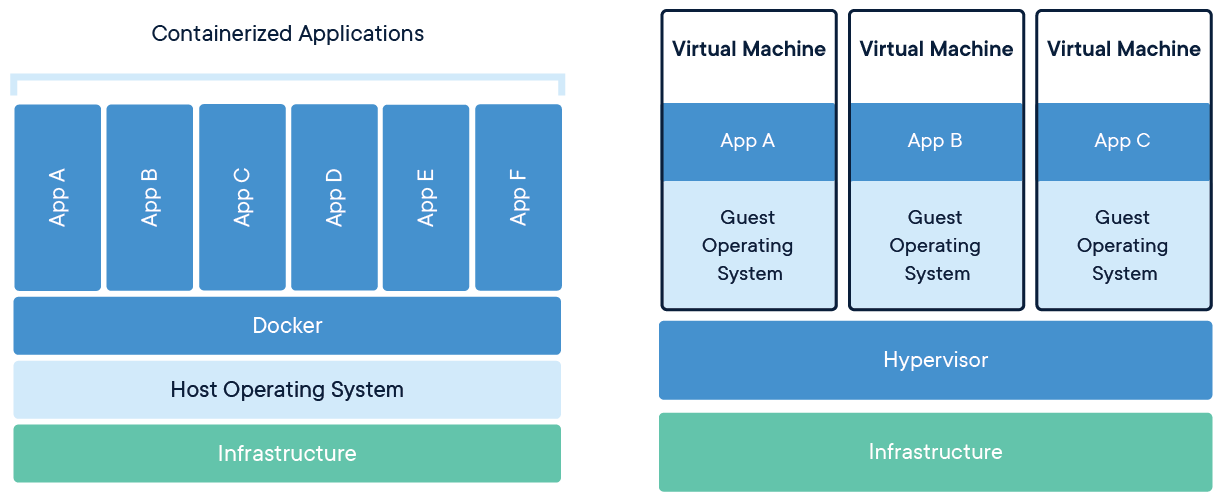
\includegraphics[width=5in]{images/Docker1}
    \caption{Virtual Machine vs Docker Container}
    \cite{dockerContainer}
\end{figure}

Docker, on the other hand, operates on top of the host OS, with applications working in tandem within the Docker platform. Another aspect of containers is that they are isolated from the host operating system and other containers and can only communicate through certain channels. An advantage that this isolation brings with it is that the container and the code stored inside are not dependent on the host OS meaning that the only requirements to run the code stored within the container are Docker and the name of the image or container. This, in a way fixes, the timeless joke of "Well, it works on my machine" by essentially allowing for a developer to ship the machine that the code was developed on.

Docker has other inherent advantages over using Virtual Machines mainly in the region of overall performance and resource use. In tests performed by MinSu Chae \cite{chae2019performance} it was found that Docker containers on a single machine outperform Virtual Machines, specifically KVM Virtual Machines in all tests that were performed by a large margin of between 3.6 to 4.6 percent. These tests focused on memory usage and CPU idle rates with at the lowest a single Docker container or Virtual Machine and highest four Docker containers or Virtual Machines. The results from these tests show the reason why the use of containerization software and platforms is slowly becoming the industry standard and the use of Virtual Machines is slowly decreasing.

There are countless other aspects of Docker from deploying a cluster of containers known as a 'swarm'. This utility can be used to ensure that a website can properly handle an increase in site traffic or have different services handled by different containers. This allows for containers to be specialized for certain tasks. This ability is also found in other tools, the most well-known one being Kubernetes which will be discussed in the Current State of the Art section \ref{sec:stateofart}.

\section{Motivation}
\label{sec:motivation}

Several events motivated me to try and create this tool as well as to become more proficient with Docker. This is an investigation based on innate curiosity and the desire to learn a new skill, as there has been a fair amount of 'buzz' within Computer Science surrounding containers and the containerization of software and software systems for a fair amount of time. However, the main push which cast me into the world of Docker was from John Abbott who is a close family friend that works for IBM and has been an on-again, off-again mentor to me. John highly suggested that I begin to look into and if possible become proficient with Docker. The reasoning behind this was from his perspective in the Computer Science industry there is a lot of movement towards containerization. Due to this, being able to demonstrate that I have some kind of rudimentary understanding and experience with Docker could make my resume more attractive to prospective employers once I began looking for a job.

This event occurred over the summer and for a short while I began to look into Docker, as well as a few other things which he suggested I take a look at but do not have any relevance. However, I quickly lost motivation due to working long days and as a result learning, Docker quickly slipped out of my mind. Once the semester began, motivation once again came, this time in the form of having to help first-year students, as well as upperclassmen, try to get Docker installed and running on their laptops. The difficulties that many of the students faced in trying to Docker to work as well as trying to figure out the differences between the version of Docker pushed me to learn as much as possible about Docker. From there I began to experiment with Docker, following the online tutorials on Docker's 'Get Started' pages to learn the basics and slowly built my understanding of how Docker worked. Eventually, I was able to make my images of incredibly simple Python programs that could receive user input or command-line arguments.

Through this process of learning the basics of Docker, I saw just how useful of a tool it can be and began to see many of the other spots where it was lacking. One of these areas was helping new users to learn the basics of Docker. The documentation online while helpful was at times overly complex and the amount of information given is not entirely necessary. This motivated me to begin to look into ways that could streamline the installation process of Docker across operating systems and create a simple interface for new users of Docker. As such, I began to look into the feasibility of such a task. In the process of exploring this, I began to wonder about automatically generating Dockerfiles. This was an area that could be incredibly useful so I tried to see if that was something that already existed and if not if it would be possible to do. After researching the feasibility of adding that component I decided that it would be and added it to the overall project.


\section{Current State of the Art}
\label{sec:stateofart}

Containerization software is slowly making its way into more and more areas in the Computer Science industry. There are many different containerization software that exists with Docker being the most well known and one of the most widely utilized. Another state of the art containerization platform that exists is Kubernetes \cite{kubernetes}, which has compatibility with some aspects of Docker and as such can be easily used interchangeably with Docker. Kubernetes has the advantage of being originally developed by Google and as such has some integrations with other Google services, like their cloud platform. Another well-known software is Microsoft's Azure \cite{azure}. This software, which is developed and maintained by Microsoft and is built off of Kubernetes. Kubernetes, while being a containerization platform acts more so as a distribution and management platform for containers as well as for coordinating clusters of Docker nodes.

\section{Goals of the Project}
\label{sec:goals}

There are several goals for this project. The first, and in my opinion, the most important goal is to gain a better understanding of Docker and how it works and can be utilized. This as previously discussed in the motivation \ref{sec:motivation} was the primary goal of looking into Docker over the summer and continues to be one of the main goals. The area of Docker and containerization is still fairly young and as such new uses and information on this topic are constantly being figured out. Due to this, there will always be something new to learn in this area, which is something that will force me to constantly learn. Being able to create Docker containers that can perform different services and run the software will hopefully reflect well in the future and as such may help in getting a job in the future.

The first tangible goal of the project is to develop a software tool that can detect the host machine's operating system and in the case of Windows and Linux the version of the OS. This will then allow for the tool to determine what the proper method to install Docker is and perform that operation. The aim of this is to allow for an easier and more streamlined installation process that can be used more universally. This as previously mentioned is due to the challenges that were faced when the Computer Science Department began to transition to the use of Docker and Docker containers in Computer Science classes.

The next goal is to develop a simple, but optimized, graphical user interface that will allow users who have no experience with Docker to learn the many command-line arguments that Docker has. Docker has forty base commands with purposes ranging from the building and creation of Docker images to removing images and containers from a given machine, which are two separate commands. Most of these forty commands are not required for an introductory user of Docker and as such can just cause further confusion with a topic that can already be intimidating when starting.

The final goal is to create a system that can be supplied with a directory that contains programs that a user wants to contain in a Docker container. This system will then determine what languages are being used and add the necessary installation commands to a Dockerfile along with adding all programs contained within the specified directory. In the end, this will create the perfect Docker container which the user can run to interact with or run the programs in the given directory.

\section{Thesis Outline}
\label{sec:outline}

The creation of this proposed tool will streamline the installation and use of Docker. Docker is an incredibly useful tool that is slowly beginning to enter more and more regions of computer science, from software to websites and web applications. As such becoming proficient with or at least having a basic understanding of how to use and utilize Docker can be a knowledge set that will be more and more useful as time goes on. The simplistic and streamlined nature of the user interface that will be proposed, will allow for introductory users of Docker to learn the basics of Docker easier. This will be due to the consolidation of the extensive command and argument list that is present in the command line operation of Docker. The proposed tool will also make it easier for the user to learn how to create Dockerfiles, which are integral to the creation and use of Docker images which are utilized by Docker containers. This aspect will be accomplished by allowing users to automatically create the Dockerfiles necessary for a given directory and learn the general structure that Dockerfiles have. The combination of these three elements of the tool, the installer, the interface, and the Dockerfile generator, will create an overall software tool that will allow a new user of Docker to more easily learn the basics.
 % Introduction (first numbered chapter)

%\numberedchapter{Related Work}
\chapter{Related Work}
\label{ch:relatedwork}

This chapter will introduce several preexisting technologies in the different areas that my tool will be focusing on. These areas are the automatic installation of Docker on a given machine, a graphical user interface for the interaction with different elements of Docker, and finally, a tool which upon being supplied with a file path to a directory will write a Dockerfile that can run any programs in that directory. It will then perform an analysis of these different components and illustrate what aspects I will be mimicking in the final tool and what elements I will improve upon.

\break

\section{Docker Installer}
\label{sec:installer}

There are several preexisting tools for automatically installing Docker onto a machine. These tools are Docker Desktop and Docker Toolbox. There are several issues with these installers. The first issue is that these installers are only for Mac OS and Windows, meaning that there is currently not an official Docker installer for Linux. These tools can be found on Docker's official website along with installation instructions and a lot more information on which someone who is just starting to learn how to use Docker, will not need it. The sheer amount of information that is present can also make figuring out what the correct installer is difficult.

This can be seen in the documented steps for installing Docker on Linux distributions which alone have five different pages for the various distributions of Linux and an additional sixth page for optional post-installation instructions \cite{dockerDocs}.

However, the biggest installation issue comes when a user tries to install Docker on Windows as there are two distinct versions of Docker for Windows, Docker Desktop for Windows Professional users and Docker Toolbox for Windows Home users. Unfortunately, both of these versions require the user to turn on Virtualization technology, which can only be done from the BIOS settings. The next issue with the Windows version comes in the form of the actual installer that is provided by Docker. This installer will sometimes install incorrect or versions of required software that are known to be buggy, mainly a version of VirtualBox is a Software tool for creating Virtual Machines and is required to use Docker on Windows.

In contrast to Windows Home, which uses the Docker Toolbox, Windows Professional uses a program called Docker Desktop, which in my experience has a much higher first-time installation success rate. The reason for this the difference in version comes down strictly to a minor difference between Windows Home and Windows Professional. This difference is the installation of Hyper-V technology, something which Microsoft allows to be installed on Windows Professional but not Windows Home, thus requiring Home users to install Docker Toolbox.

Mac OS users have it much easier as there is only a single install for the operating system which when run will install Docker correctly. There is the bonus of Mac OS being a Unix based system so if a user installs Homebrew, they can use the command line to interact with Docker and not have to rely on graphical interfaces if they prefer to use the command line.

\section{Docker Interface}
\label{sec:interface}

There are currently several graphical interfaces available for the creation and management of Docker containers. One of these interfaces comes directly from Docker and is known as Kitematic \cite{kitematic}, which has the added advantage of being officially supported by the developers of Docker. This will allow for Kitematic to stay up to date with any changes that Docker may make and in theory, would allow it to be the best interface This program, however, is only available for Mac OS and Windows and will not run on Linux distributions. Looking at the interface itself, however, illustrates the amount of time that Docker Inc. has placed into making sure that the interface is usable. This is because the interface is overall very simple and clean looking, there is not a lot of extraneous text or options and it allows for a user to easily download an image from Docker Hub and have a container running. From there Kitematic also includes an in interface terminal for interaction with containers which allows for Kitematic to be a 'one-stop-shop' for Docker users. However, while this may make using Docker easier for anyone to use it does not necessarily allow for a user to learn the backend aspects of building and running an image and/or a container.

\begin{figure}[h!]
    \centering
    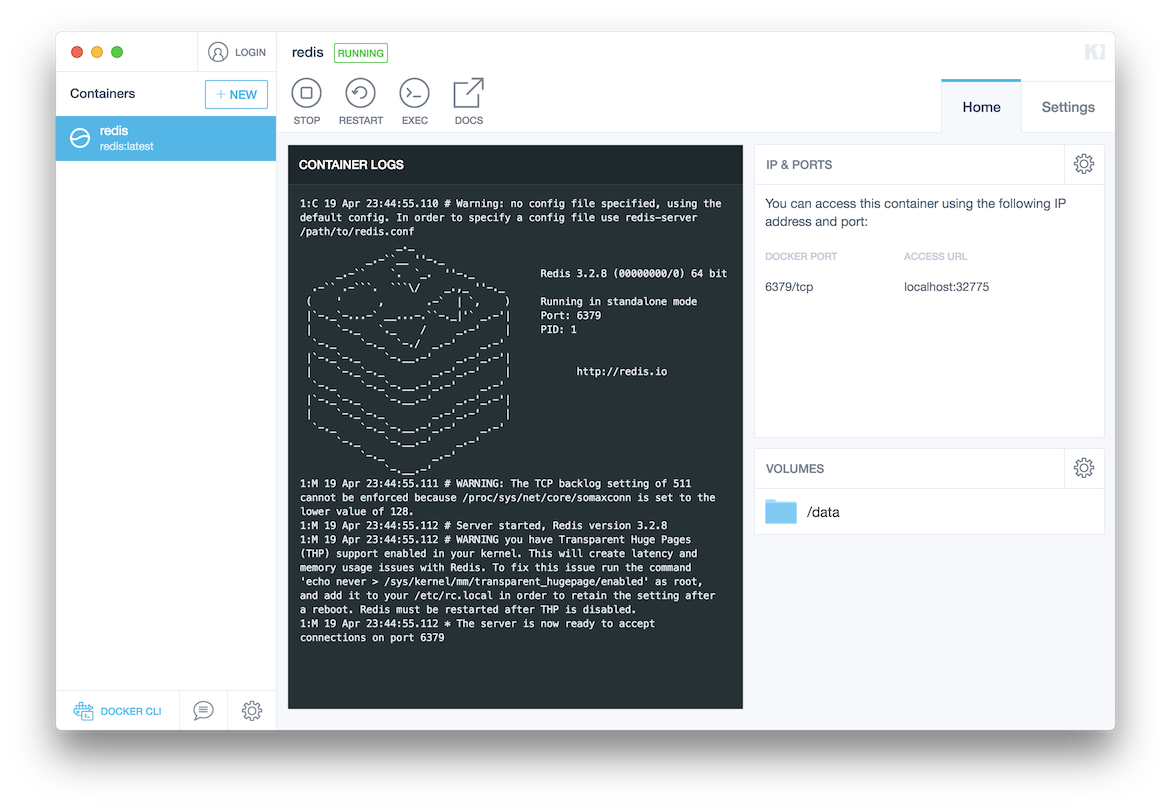
\includegraphics[width=5in]{images/Kitematic}
    \caption{Kitematic Dashboard}
\end{figure}

The main limitations of Kitematic, not supporting all operating systems, are not found in other interfaces like DockStation, which supports Linux as well as Mac OS and Windows. However, DockStation \cite{dockstation} does not install any form of Docker along with itself and as such requires a successful installation before it can be utilized. Another limitation of DockStation is that it requires the use of Docker Compose, which is an additional installation which is not included in the base Docker for Linux. An additional limitation of DockStation is it does not allow for the running of Docker images, only Docker containers. This, in turn, does not allow for a user to use the '--rm' command line flag when running an image that deletes the resulting container upon exiting the container. Dockstation also has additional tools that allow for the monitoring of local and remote Docker containers and other utilities that are aimed more at higher level users of Docker. Among the information provided is the current status of the container as well as all logs that are created in the process of it running.

\begin{figure}[h!]
    \centering
    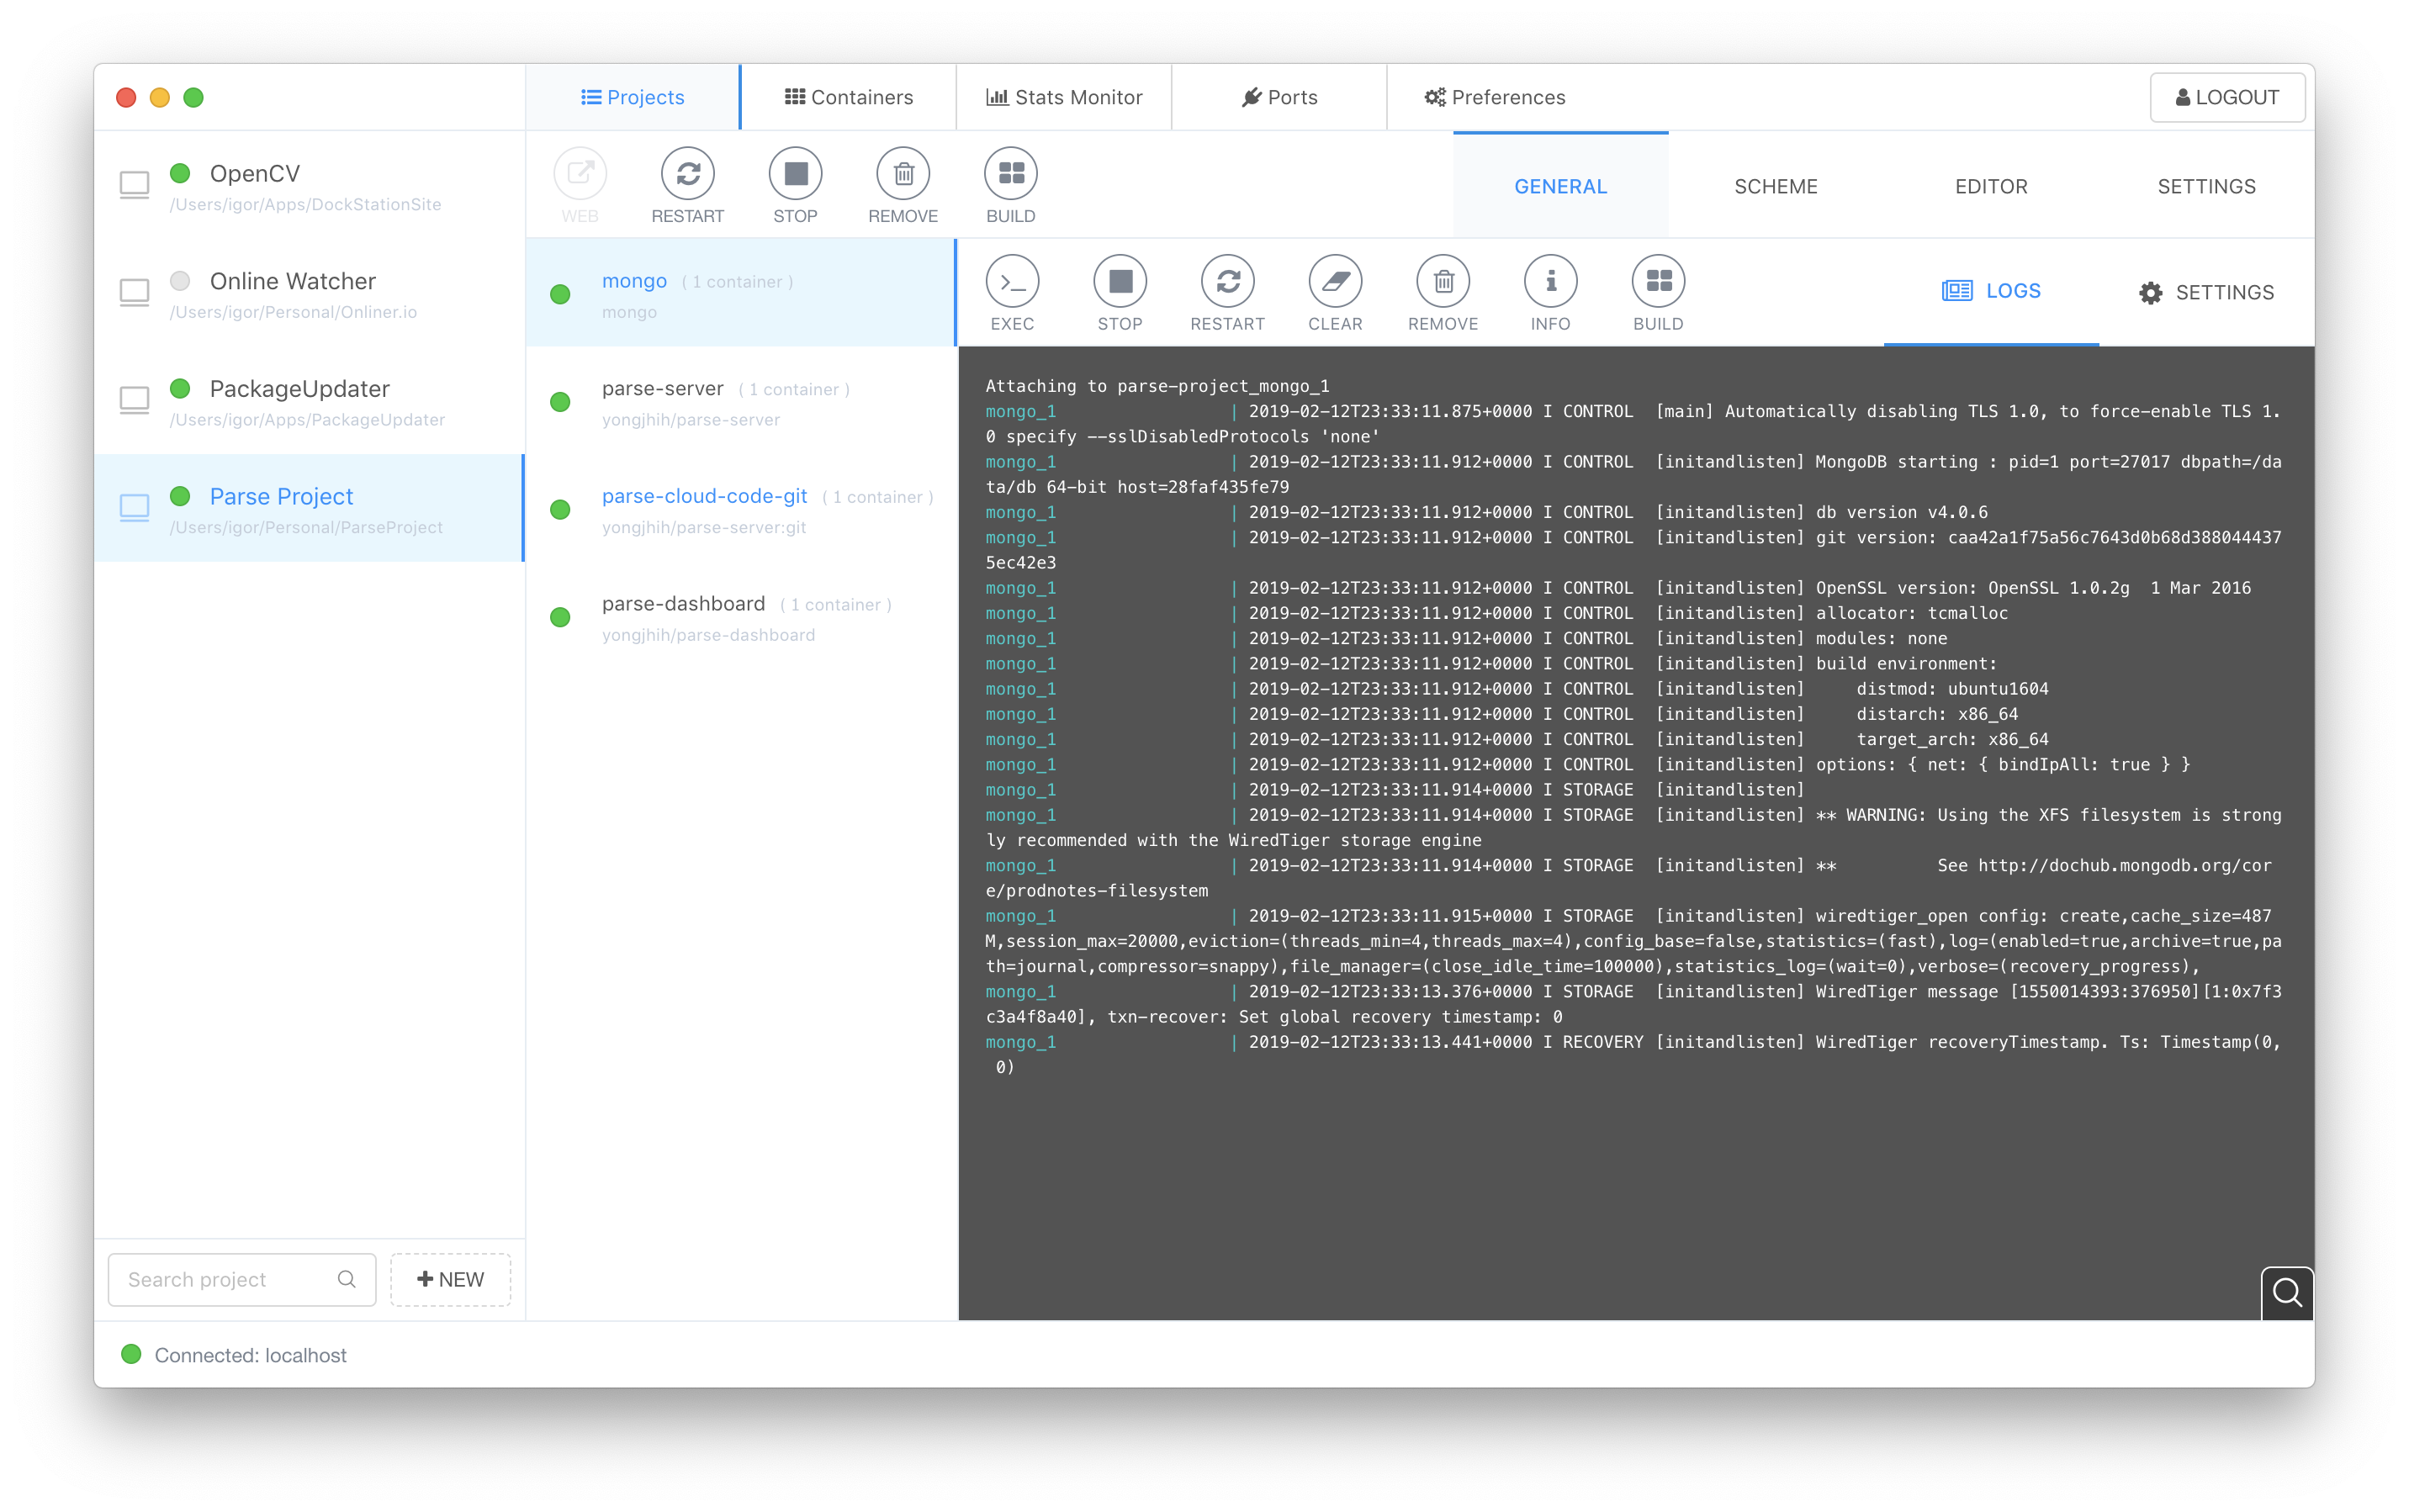
\includegraphics[width=5in]{images/DockStation}
    \caption{DockStation Interface}
\end{figure}

A graphical interface that works well and looks good is Portainer \cite{portainer}, this interface is a web-based application and allows for the creation and running of images and containers. However, the largest limitation with Portainer is that it requires Docker for it to be run and does not install Docker alongside itself like Kitematic. Portainer also has many features that DockStation does, like the remote monitoring of containers that are running and a system for easily creating containers quickly and easily. Despite requiring Docker to run, Portainer has a very intuitive interface that I will base my interface on. The simplistic nature of the overall tool makes it easy to figure out. It also is a rather lightweight application and only requires enough memory to run due to it running inside of a Docker container. However, I will not include some of the elements that I deem to be not needed or even redundant like networks, which for an introductory level Docker interface is not necessary.

\begin{figure}[h!]
    \centering
    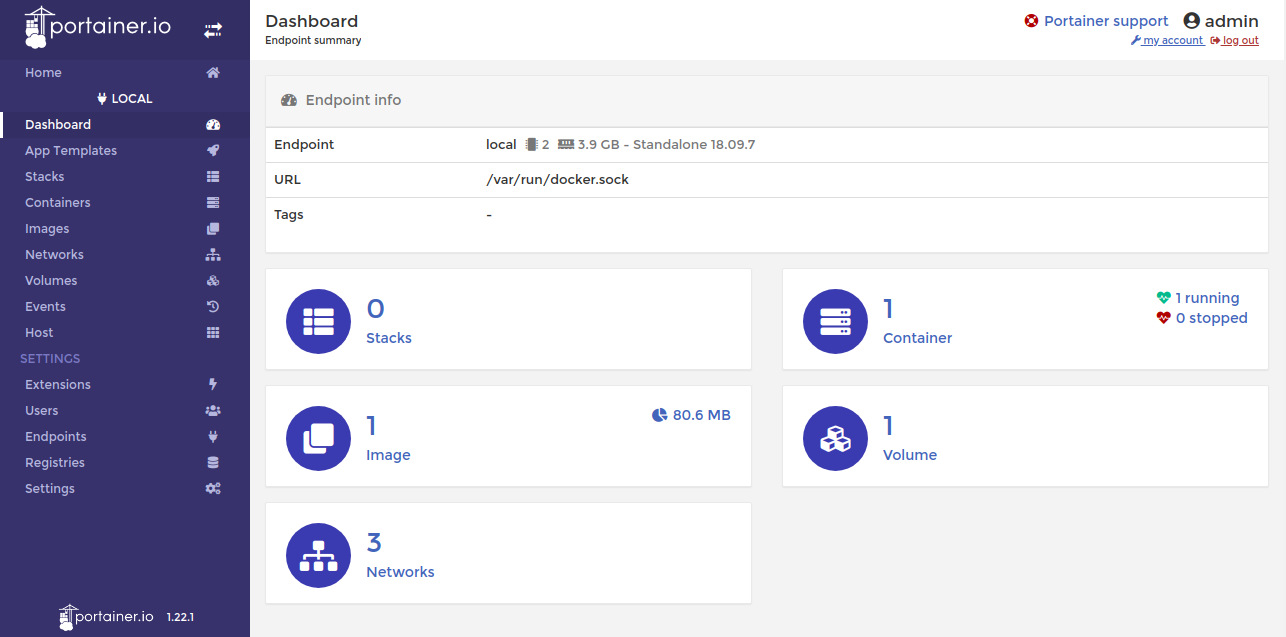
\includegraphics[width=5in]{images/Portainer}
    \caption{Portainer Dashboard}
\end{figure}

\section{Dockerfile Generator}
\label{sec:generator}

Tools that help the user to generate a Dockerfile are not very common due to the sheer number of ways that a Dockerfile can be written to accomplish the same task. However, in my search, I was able to find a single tool that had similarities to what I hope to accomplish, Microsoft's Generator-docker for Linux terminals \cite{microsoft_2018}. This tool, which was written in JavaScript allows for a user to specify the language of the project that they want to be run in the container along with several other factors, like the name of the image and the port, the application will be listening to.

However, this tool has many limitations. The first limitation is that the process is not automatic, the user has to specify the language that the container will use and there can only be a single language specified. Along the lines of programming language, this tool only supports three languages, .NET Core, Node.js, and Golang, which does allow for a closer degree of customization of the Dockerfile but does create a limitation in the number of projects that would be supported. This aspect is something that will, hopefully, not be a part of the generator tool that I create.

This tool, on the other hand, does have features that will be a part of or similar to features in the final Dockerfile generator which I create. The main feature which will be present is a way for a user to build and run their Docker image after the creation of the Dockerfile. This feature will not necessarily be a part of the generator and will instead be a feature of the graphical interface. With Generator-docker this code is contained and ran by a separate program written in bash that is automatically generated by the generator. Where my tool will differ from this approach is instead of creating a separate program that can be used to build and run the image, the graphical interface will have the option to build the image as well as to run a specified image.

\section{Overall Tool}
\label{sec:overall}

There are currently no tools available which combine all three aspects of the tool that I will be creating. A slight exception to this is the interface Kitematic which was mentioned in the Interface section \ref{sec:interface}. This is an interface, as previously mentioned, that has been developed by Docker and as such Kitematic is included with Docker Toolbox and Docker Desktop. However, due to this fact if a user faces any issues when trying to install Docker then the inclusion of the Kitematic interface is useless. Due to the lack of all in one tool in this overall area of Docker tools the development of the tool that I will be creating will greatly benefit the Docker community.


%\numberedchapter{Method Of Approach}
\chapter{Method of Approach}
\label{ch:method}

This chapter will focus on the implementation of the software tool initially proposed in Chapter \ref{ch:intro}. The overall software is composed of three separate tools, an installer, an interface, and a Dockerfile generator. The primary language used for this project is Python due to packages available within Python and the ease to add and import external packages. Two main packages are being utilized for the creation of the tool which is the Docker Python \cite{dockerPython} wrapper for interacting with Docker and Flask \cite{flask} for building the browser-based interface.

\break

% This chapter should answer the ``how'' question - how did you complete your project, including the overall design of your study, details of the algorithms and tools you have used, etc.
%  Use technical diagrams, equations, algorithms, and paragraphs of text to
% describe the research that you have completed. Be sure to number all figures and tables and to explicitly refer to them in your text.

The software tool, that I have developed, as previously mentioned has three main components. The Docker Installer, the Interface, and the Dockerfile Generator. Each of these components works together to ensure optimum user experience. The installer ensures that the user will be able to properly use Docker, the Interface, and the Dockerfile Generator. The Interface allows the user to easily use the Dockerfile Generator and interact with the more common Docker commands. The Dockerfile Generator allows the user to easily create Docker images that the Interface can run. The overall file structure of the tool can be seen in Figure \ref{fig:fileStruct} below.

\begin{figure}[h!]
  \dirtree{%
.1 Docker-Automation/.
.2 auto/\DTcomment{Main Utilities and Program Files}.
.3 containers\DTcomment{Container Utilities Program File}.
.3 docker\_auto\DTcomment{Command Line Interface Program File}.
.3 generate\DTcomment{Dockerfile Generator Program File}.
.3 images\DTcomment{Image Utilities Program File}.
.3 install\DTcomment{Installation Functions Program File}.
.2 interface/\DTcomment{Flask Interface and Style Files}.
.3 static/\DTcomment{Static Files Used for Interface Construction}.
.3 templates/\DTcomment{HTML Pages for Interface}.
.3 interface\_containers\DTcomment{Containers Interface Utilities Page}.
.3 interface\_main\DTcomment{Main Interface Page}.
.3 interface\_images\DTcomment{Images Interface Utilities Page}.
.2 tests/\DTcomment{Tests to Ensure Utilities Function Properly}.
.2 samples/\DTcomment{Test Directories to Ensure Generator Functions Properly}.
.2 evaluator/\DTcomment{Evaluation Suite}.
.3 data\DTcomment{Data Aggregator and Processor}.
.3 evaluate\_build\DTcomment{Evaluation Tests for Image Building}.
.3 evaluate\_generate\DTcomment{Evaluation Tests for Dockerfile Generation}.
.3 evaluate\_install\DTcomment{Evaluation Tests for Docker Installation}.
.3 evaluate\_run\DTcomment{Evaluation Tests for Image Running}.
.3 output\DTcomment{Data Output File}.
.2 main\DTcomment{Tool Driver File}.
.2 eval\DTcomment{Evaluation Driver File}.
}

  \caption{Docker Automation File Structure}
  \label{fig:fileStruct}
\end{figure}

% \break

\section{Utilized Tools}
\label{sec:tools}

To develop this tool, as previously mentioned, I utilized several APIs and packages. The first and one of the most important of these was the Python Docker API which gave access to Docker commands within Python programs. This process could have been performed in other ways, like executing each command via the Python OS package, however, this method did not have a guarantee to work on every operating system due to differences in how Docker operates on each.

The next most important package utilized was Python Flask \cite{flask}. This package allows for the creation of webpages utilizing endpoints for executing different functions. This package was utilized to create the user interface due to web browsers being more universal on different operating systems. Another advantage of utilizing Flask is that it also creates the web server in which the interface is run on. This decreases the number of required packages for the overall software tool.

An additional tool that was used is Pipenv \cite{pipenv}. This was used for its ability to manage the required packages and environment setup. Pipenv is similar to Python's Pip package manager, which was initially used before switching to Pipenv. This switch was made for a variety of reasons the first of which was its inclusion of a virtual environment for development. The second reason was due to its built-in requirements manager. This came in the form of Pipfiles which keep track of each package that is installed. This method is far more desirable rather than Pip's requirements.txt format of keeping track of requirements due to the automation of its creation.

The final tool that was utilized was Pytest \cite{pytest}, a package that can be used to write helpful test cases which can ensure that a program is functioning correctly even after changes to the code. This tool was useful to a degree in ensuring that different functions were still generating the expected output or results, though in some cases tests were not entirely feasible or convenient. However, Pytest was very useful after refactoring the basic code for the different utilities as there were several times in which certain functions were not tested by myself and as a result, any issues with them went unnoticed. With the addition of utilizing Travis-CI, a continuous integration service, these tests were run each time changes were made within the repository of the tool and ensured that any issues were quickly identified and fixed.

\section{Installer}
\label{sec:installer}

The Installer has multiple procedures it runs to ensure that Docker will successfully install on a given machine. The first procedure that is run is determining the operating system that the machine is running. For this, I utilized a python package called Platform, which has many useful methods for retrieving system information, like the operating system type. Once the operating system is determined the next step is to figure out the exact version that is being run. This is more important for operating systems like Linux and Windows than with Mac OS due to the different versions of each of those systems having different installation requirements and commands.

Once the specific version, or in the case of Linux based systems Distribution, has been determined the next step is to load and run the installation instructions. As of writing this the only instruction sets that have been tested and verified to work correctly are the Linux based systems, ie Ubuntu, Fedora, Debian, and CentOS. Instruction sets do exist for Windows and Mac OS, however, these platforms have not yet been tested due to focusing on ensuring that other portions of the system were properly working for Linux systems.

Once the instruction set is loaded each command is then run utilizing Python's built-in OS package and the system method. This method allows for a Python script to run commands on the machine outside of Python. Once this step has been completed the installer will then execute a simple Docker command to test if the installation was a success or not. The chosen command is 'Docker run hello-world', which not only checks if Docker has been installed correctly but also if the machine can retrieve images from external sources.

The overall installation described below can be seen in figure \ref{fig:install}, which generalizes the installation process down to its core elements. The pseudocode for the installation process can also be seen in Algorithm \ref{alg:install}. The installation process utilizes three main functions that perform different steps to aid the installation process. The main function, install, handles the back and forth between the two other functions, get\_instructions and execute\_instructions. Install also handles determining the operating system, and if necessary the distribution. This information is passed to get\_instructions which maps the operating system to a corresponding instruction set file path. This path is then passed to execute\_instructions which loads the instruction set and executes each command. If there are no issues in execution, the function returns True, however, if any issues are faced it returns False. After this a final function, confirm\_installation, is called to ensure that Docker has been installed. This is performed by simply running the Docker hello\-world image and checking if any errors are raised upon attempting to do so.


\begin{figure}[h!]
  \centering
  \begin{center}
\end{center}
\tikzset{every picture/.style={line width=0.75pt}} %set default line width to 0.75pt
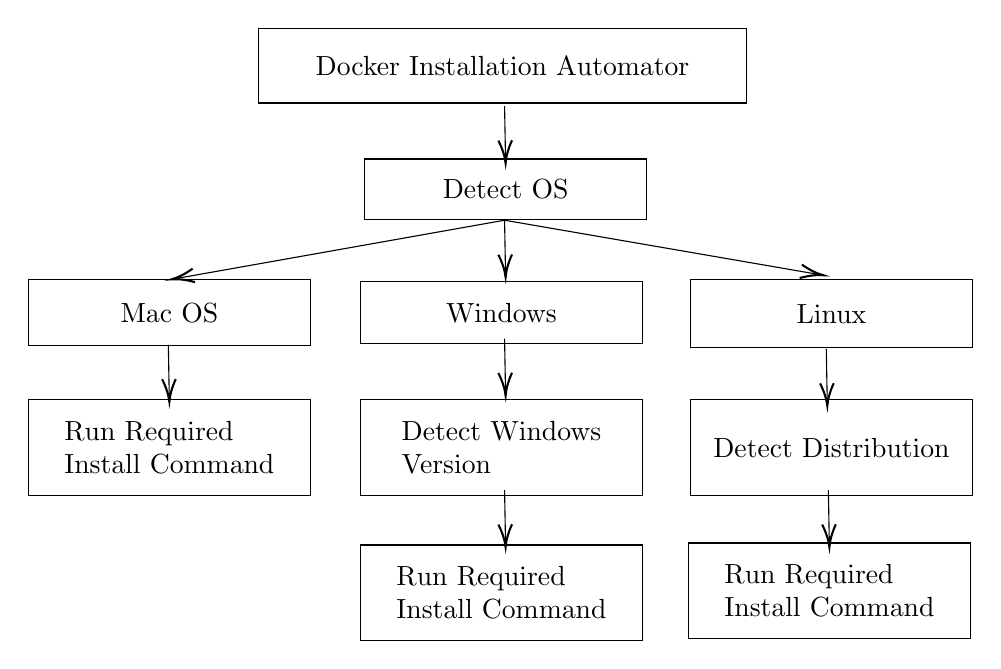
\begin{tikzpicture}[x=0.75pt,y=0.75pt,yscale=-1,xscale=1]
%uncomment if require: \path (0,387); %set diagram left start at 0, and has height of 387
%Shape: Rectangle [id:dp12391033482252478]
\draw   (232.5,102) -- (368.5,102) -- (368.5,131) -- (232.5,131) -- cycle ;
%Shape: Rectangle [id:dp2555094989002722]
\draw   (181.5,39) -- (416.5,39) -- (416.5,75) -- (181.5,75) -- cycle ;
%Shape: Rectangle [id:dp03162657543059133]
\draw   (70.5,160) -- (206.5,160) -- (206.5,192) -- (70.5,192) -- cycle ;
%Shape: Rectangle [id:dp1947521533199792]
\draw   (230.5,161) -- (366.5,161) -- (366.5,191) -- (230.5,191) -- cycle ;
%Shape: Rectangle [id:dp39981703441594085]
\draw   (389.5,160) -- (525.5,160) -- (525.5,193) -- (389.5,193) -- cycle ;
%Shape: Rectangle [id:dp5445432499512475]
\draw   (389.5,218) -- (525.5,218) -- (525.5,264) -- (389.5,264) -- cycle ;
%Shape: Rectangle [id:dp16820618798873133]
\draw   (388.5,287) -- (524.5,287) -- (524.5,333) -- (388.5,333) -- cycle ;
%Shape: Rectangle [id:dp200391241880703]
\draw   (230.5,288) -- (366.5,288) -- (366.5,334) -- (230.5,334) -- cycle ;
%Shape: Rectangle [id:dp30770436978288385]
\draw   (230.5,218) -- (366.5,218) -- (366.5,264) -- (230.5,264) -- cycle ;
%Shape: Rectangle [id:dp693797802592405]
\draw   (70.5,218) -- (206.5,218) -- (206.5,264) -- (70.5,264) -- cycle ;
%Straight Lines [id:da8290451967136283]
\draw    (300,76.5) -- (300.46,102) ;
\draw [shift={(300.5,104)}, rotate = 268.96] [color={rgb, 255:red, 0; green, 0; blue, 0 }  ][line width=0.75]    (10.93,-3.29) .. controls (6.95,-1.4) and (3.31,-0.3) .. (0,0) .. controls (3.31,0.3) and (6.95,1.4) .. (10.93,3.29)   ;
%Straight Lines [id:da46504760658282174]
\draw    (300,131.5) -- (300.46,157) ;
\draw [shift={(300.5,159)}, rotate = 268.96] [color={rgb, 255:red, 0; green, 0; blue, 0 }  ][line width=0.75]    (10.93,-3.29) .. controls (6.95,-1.4) and (3.31,-0.3) .. (0,0) .. controls (3.31,0.3) and (6.95,1.4) .. (10.93,3.29)   ;
%Straight Lines [id:da697562345132964]
\draw    (300,188.5) -- (300.46,214) ;
\draw [shift={(300.5,216)}, rotate = 268.96] [color={rgb, 255:red, 0; green, 0; blue, 0 }  ][line width=0.75]    (10.93,-3.29) .. controls (6.95,-1.4) and (3.31,-0.3) .. (0,0) .. controls (3.31,0.3) and (6.95,1.4) .. (10.93,3.29)   ;
%Straight Lines [id:da29460818271989786]
\draw    (300,261.5) -- (300.46,287) ;
\draw [shift={(300.5,289)}, rotate = 268.96] [color={rgb, 255:red, 0; green, 0; blue, 0 }  ][line width=0.75]    (10.93,-3.29) .. controls (6.95,-1.4) and (3.31,-0.3) .. (0,0) .. controls (3.31,0.3) and (6.95,1.4) .. (10.93,3.29)   ;
%Straight Lines [id:da12315236334431812]
\draw    (455,193.5) -- (455.46,219) ;
\draw [shift={(455.5,221)}, rotate = 268.96] [color={rgb, 255:red, 0; green, 0; blue, 0 }  ][line width=0.75]    (10.93,-3.29) .. controls (6.95,-1.4) and (3.31,-0.3) .. (0,0) .. controls (3.31,0.3) and (6.95,1.4) .. (10.93,3.29)   ;
%Straight Lines [id:da4360797681426818]
\draw    (138,191.5) -- (138.46,217) ;
\draw [shift={(138.5,219)}, rotate = 268.96] [color={rgb, 255:red, 0; green, 0; blue, 0 }  ][line width=0.75]    (10.93,-3.29) .. controls (6.95,-1.4) and (3.31,-0.3) .. (0,0) .. controls (3.31,0.3) and (6.95,1.4) .. (10.93,3.29)   ;
%Straight Lines [id:da47355294652329594]
\draw    (456,261.5) -- (456.46,287) ;
\draw [shift={(456.5,289)}, rotate = 268.96] [color={rgb, 255:red, 0; green, 0; blue, 0 }  ][line width=0.75]    (10.93,-3.29) .. controls (6.95,-1.4) and (3.31,-0.3) .. (0,0) .. controls (3.31,0.3) and (6.95,1.4) .. (10.93,3.29)   ;
%Straight Lines [id:da6592684678579579]
\draw    (300,131.5) -- (451.53,157.66) ;
\draw [shift={(453.5,158)}, rotate = 189.79] [color={rgb, 255:red, 0; green, 0; blue, 0 }  ][line width=0.75]    (10.93,-3.29) .. controls (6.95,-1.4) and (3.31,-0.3) .. (0,0) .. controls (3.31,0.3) and (6.95,1.4) .. (10.93,3.29)   ;
%Straight Lines [id:da5603048049658739]
\draw    (300,131.5) -- (141.47,159.65) ;
\draw [shift={(139.5,160)}, rotate = 349.93] [color={rgb, 255:red, 0; green, 0; blue, 0 }  ][line width=0.75]    (10.93,-3.29) .. controls (6.95,-1.4) and (3.31,-0.3) .. (0,0) .. controls (3.31,0.3) and (6.95,1.4) .. (10.93,3.29)   ;
% Text Node
\draw (299,57) node  [align=left] {Docker Installation Automator};
% Text Node
\draw (300.5,116.5) node  [align=left] {Detect OS};
% Text Node
\draw (138.5,176) node  [align=left] {Mac OS};
% Text Node
\draw (298.5,176) node  [align=left] {Windows};
% Text Node
\draw (457.5,176.5) node  [align=left] {Linux};
% Text Node
\draw (457.5,241) node  [align=left] {Detect Distribution};
% Text Node
\draw (456.5,310) node  [align=left] {Run Required\\Install Command};
% Text Node
\draw (298.5,311) node  [align=left] {Run Required\\Install Command};
% Text Node
\draw (298.5,241) node  [align=left] {Detect Windows\\Version};
% Text Node
\draw (138.5,241) node  [align=left] {Run Required\\Install Command};
\end{tikzpicture}

  \caption{Automated Docker Installation Process}
  \label{fig:install}
\end{figure}

\begin{algorithm}[H]
  \SetKwInOut{Input}{input}
\SetKwInOut{Output}{output}
\SetKwProg{Fn}{Function}{}{end}
\Fn{install()}{
  \Output{A message of if Docker is properly installed}
  $OS\leftarrow$platform.system() \\
  \uIf{OS == Linux}{
    $distro\leftarrow$platform.linux\_distribution()
  }
  \uElseIf{OS == Mac OS}{
    $distro\leftarrow$MacOS
  }
  \uElseIf{OS == Windows}{
    $distro\leftarrow$Windows
  }
  $file\leftarrow$get\_instructions($distro$)\\
  execute\_instructions($file$)
}
\SetKwProg{Fn}{Function}{}{end}
\Fn{get\_instructions($distro$)}{
  \Input{$distro\leftarrow$ The name of the instruction set to load}
  \Output{$file\leftarrow$ Filepath to the corresponding instruction set for $distro$}
  \If{$distro$ == distro\_name}{
    $file\leftarrow$ $file\_path$
  }
  return $file$
}
\SetKwProg{Fn}{Function}{}{end}
\Fn{execute\_instructions($file$)}{
  \Input{$file$: The path to the instruction set for the host machine}
  \Output{True or False, corresponding to if there are any issues faced during command execution}
  $commands\leftarrow$open($file$, \'r\')
  \For{$command$ in $commands$}{
    os.system($command$)
    \If{Issue faced}{
      return $False$
    }
  }
  return $True$
}
\Fn{confirm\_installation()}{
  $installed\leftarrow$ $False$ \\
  docker run $hello-world$ \\
  \If{No Issues}{
    $installed\leftarrow$ $True$
  }
  return $installed$
}

  \caption{Installation Algorithm Pseudo Code}
  \label{alg:install}
\end{algorithm}


\section{Interface}
\label{sec:interface}

The goal of the interface is to streamline the user experience interacting with the more common Docker elements like running and deleting both Docker containers and Docker images. Another goal is to have the interface be visually appealing to allow for extended use of the interface.

The Interface itself utilizes a combination of HTML, CSS, JavaScript, and the Python Flask \cite{flask} framework to create the interface as a webpage that can be viewed in any web browser. This switch from utilizing a direct GUI package as described in the Proposal is due in part to the goal of ensuring that this system will be able to work with nearly every operating system. An additional reason for the switch between a dedicated GUI and Flask is the ease of developing the interface itself. With many of the GUI packages, I researched the level of customization and design was not very high, added to this was the level of difficulty that I would have faced trying to get every element to work properly and be located within the correct area.

The Interface is broken up into several different pages for the different types of functions. The first page is for functions dedicated to the creation, management, and running of Docker images. This includes a function to generate a Dockerfile for a given directory utilizing the Dockerfile Generator tool included. The next page is for functions dedicated to the creation, management, and running of Docker containers. For each page, the different functions utilize forms to submit any required information to the Flask endpoints utilizing Post methods. There is also a button on the sidebar which allows the user to shut down the tool from the interface. Images of the two main pages of the Interface, one for Images and the other for Containers can be seen below in image \ref{img:ImagesPage}.

\begin{figure}[h!]
  \centering
  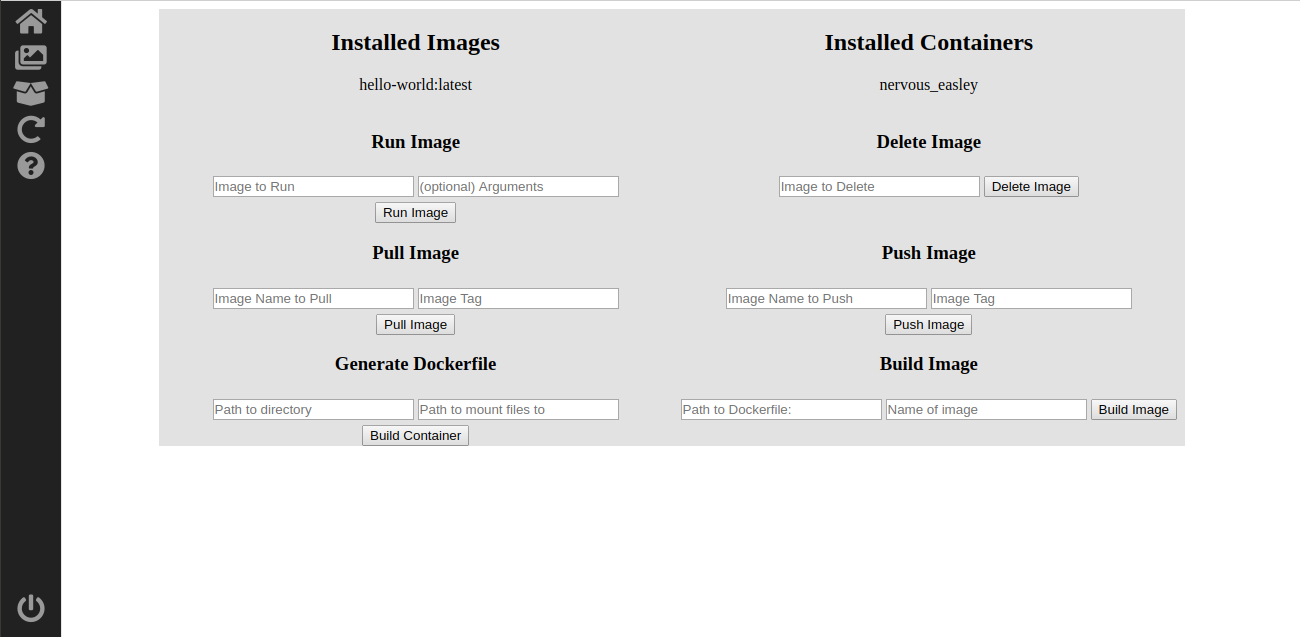
\includegraphics[width=5in]{images/InterfaceImages}
  \caption{Interface Images Page}
  \label{img:ImagesPage}
\end{figure}

Other than the visual interface there is also a command-line that can be used to interact with Docker. This aspect was included for cases where a browser-based interface may not be practical or necessary. It was also created to test functions as they were developed and instead of removing it was integrated into the overall tool. The command line has all of the same functions as the interface and can be more responsive due to not having to wait for a page to finish loading in the browser.


\section{Generator}
\label{sec:generator}

The Dockerfile Generator relies on several assumptions to work properly. These assumptions do not necessarily hurt the user's experience though with more advanced users of Linux could, in theory, have some sort of effect. The first assumption that the generator makes is that after being pointed to a directory on the host machine that the user would like to make it so that every program file within the directory is runnable. This assumption is made to decrease the number of choices that the user has to make and in doing so has a higher degree of automation for the process. Another assumption made in this regard is that if a user has multiple types of programs in the same file, they will at some point want to run each of those program files.

The next assumption that the Generator makes is that the user will not care what distribution of Linux the image is built on top of. The image the Dockerfile and the subsequent image is based on is Debian:Bullseye, which like Ubuntu, the Linux distro that I am most familiar with, uses the Apt package manager. This assumption is currently hardcoded into the Dockerfile Generator, though in the future it could be possible to modify the Generator to allow further customization of which distribution the image is based on.

The hard coding of the distribution used for the Generator is what ensures that the generator knows what package to download and install for each language. This is necessary due to there not being a default naming scheme across package managers, nor a centralized list of available packages for every programming language and package manager. As of February 28th, the Generator supports the installation of several programming languages. This list consists of Python, Java, Ruby, C, C\#, Go, JavaScript (Node.js), though adding new languages is easy to do.

\begin{figure}[h!]
  \centering
  


\tikzset{every picture/.style={line width=0.75pt}} %set default line width to 0.75pt

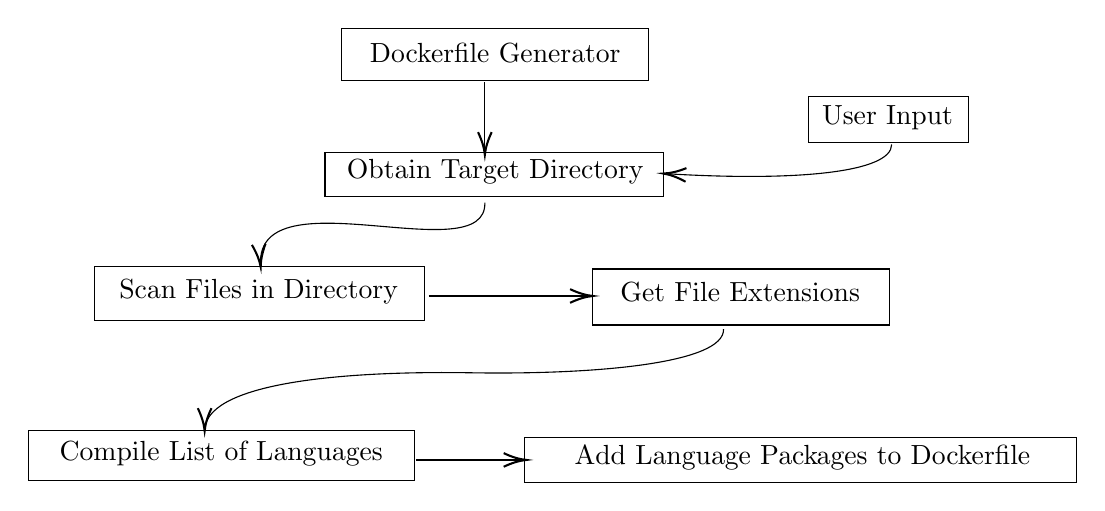
\begin{tikzpicture}[x=0.75pt,y=0.75pt,yscale=-1,xscale=1]
%uncomment if require: \path (0,447); %set diagram left start at 0, and has height of 447

%Shape: Rectangle [id:dp6708330246204339]
\draw   (254,19) -- (402,19) -- (402,44) -- (254,44) -- cycle ;
%Shape: Rectangle [id:dp3690663496827087]
\draw   (246,79) -- (409,79) -- (409,100) -- (246,100) -- cycle ;
%Shape: Rectangle [id:dp04032174080708906]
\draw   (479,52) -- (556,52) -- (556,74) -- (479,74) -- cycle ;
%Shape: Rectangle [id:dp3663336326705653]
\draw   (135,134) -- (294,134) -- (294,160) -- (135,160) -- cycle ;
%Shape: Rectangle [id:dp1296990044512687]
\draw   (375,135) -- (518,135) -- (518,162) -- (375,162) -- cycle ;
%Shape: Rectangle [id:dp5900699675454877]
\draw   (103,213) -- (289,213) -- (289,237) -- (103,237) -- cycle ;
%Shape: Rectangle [id:dp5669318997590742]
\draw   (342,216) -- (608,216) -- (608,238) -- (342,238) -- cycle ;
%Straight Lines [id:da9499154626346906]
\draw    (323,45) -- (323,78) ;
\draw [shift={(323,80)}, rotate = 270] [color={rgb, 255:red, 0; green, 0; blue, 0 }  ][line width=0.75]    (10.93,-3.29) .. controls (6.95,-1.4) and (3.31,-0.3) .. (0,0) .. controls (3.31,0.3) and (6.95,1.4) .. (10.93,3.29)   ;
%Curve Lines [id:da07473585010478478]
\draw    (519,75) .. controls (519,88.37) and (473.92,92.91) .. (410.91,89.12) ;
\draw [shift={(409,89)}, rotate = 363.58000000000004] [color={rgb, 255:red, 0; green, 0; blue, 0 }  ][line width=0.75]    (10.93,-3.29) .. controls (6.95,-1.4) and (3.31,-0.3) .. (0,0) .. controls (3.31,0.3) and (6.95,1.4) .. (10.93,3.29)   ;
%Curve Lines [id:da3255234731100256]
\draw    (323,103) .. controls (323.99,136.66) and (213.25,88.97) .. (214.91,132.65) ;
\draw [shift={(215,134)}, rotate = 265.03] [color={rgb, 255:red, 0; green, 0; blue, 0 }  ][line width=0.75]    (10.93,-3.29) .. controls (6.95,-1.4) and (3.31,-0.3) .. (0,0) .. controls (3.31,0.3) and (6.95,1.4) .. (10.93,3.29)   ;
%Straight Lines [id:da9168787921818711]
\draw    (296,148) -- (373,148) ;
\draw [shift={(375,148)}, rotate = 180] [color={rgb, 255:red, 0; green, 0; blue, 0 }  ][line width=0.75]    (10.93,-3.29) .. controls (6.95,-1.4) and (3.31,-0.3) .. (0,0) .. controls (3.31,0.3) and (6.95,1.4) .. (10.93,3.29)   ;
%Curve Lines [id:da18630293162808487]
\draw    (438,164) .. controls (438.48,180.4) and (377,186) .. (316,185) .. controls (256.52,184.03) and (191.35,189.42) .. (188.12,211.29) ;
\draw [shift={(188,213)}, rotate = 270] [color={rgb, 255:red, 0; green, 0; blue, 0 }  ][line width=0.75]    (10.93,-3.29) .. controls (6.95,-1.4) and (3.31,-0.3) .. (0,0) .. controls (3.31,0.3) and (6.95,1.4) .. (10.93,3.29)   ;
%Straight Lines [id:da8834662262571595]
\draw    (290,227) -- (341,227) ;
\draw [shift={(343,227)}, rotate = 180] [color={rgb, 255:red, 0; green, 0; blue, 0 }  ][line width=0.75]    (10.93,-3.29) .. controls (6.95,-1.4) and (3.31,-0.3) .. (0,0) .. controls (3.31,0.3) and (6.95,1.4) .. (10.93,3.29)   ;

% Text Node
\draw (328,31) node   [align=left] {Dockerfile Generator};
% Text Node
\draw (328,88) node   [align=left] {Obtain Target Directory};
% Text Node
\draw (517,62) node   [align=left] {User Input};
% Text Node
\draw (214,146) node   [align=left] {Scan Files in Directory};
% Text Node
\draw (446,146) node   [align=left] {Get File Extensions};
% Text Node
\draw (196,224) node   [align=left] {Compile List of Languages};
% Text Node
\draw (476,226) node   [align=left] {Add Language Packages to Dockerfile};


\end{tikzpicture}

  \caption{Dockerfile Generation Process}
  \label{fig:generator}
\end{figure}

\begin{algorithm}[H]
  \SetKwInOut{Input}{input}
\SetKwInOut{Output}{output}
\SetKwProg{Fn}{Function}{}{end}
\Fn{generate\_dockerfile($directory$, $to\_dir$ \= "project/")}{
  \Input{The directory to generate the Dockerfile for and optionally where to place the files to be run in the container}
  \Output{A Dockerfile which installs all required languages}

  $FILE\_TYPES\leftarrow$Dictionary of langauge packages and language extensions

  $extensions\leftarrow$get\_file\_types($directory$) \\
  \For{$ext$ in $extensions$}{
    $installs$ += FILE\_TYPES[$ext$]
  }
  Write Dockerfile with included $installs$
}

\SetKwProg{Fn}{Function}{}{end}
\Fn{get\_file\_types($directory$)}{
  \Input{The directory to analyze for file types}
  \Output{A Set of filetypes extensions found in $directory$}
  $filetypes\leftarrow$Set\\
  \For{file in $directory$}{
    $filetypes\leftarrow$file extension
  }
return $filetypes$
}

  \caption{Generator Algorithm Pseudocode}
  \label{alg:generate}
\end{algorithm}

The Generator itself works by scanning the inputted directory for files. Each file is then checked for a filetype. This is where the third main assumption is made, the Generator currently assumes that every program file utilizes a standard file extension to denote its language. In other words, Python files end with .py (and are written in Python3, though due to an upcoming depreciation of Python2 is not an invalid assumption) and Java files end with .java. This assumption is not necessarily bad, though having methods that analyze the contents of the file, especially in the case of there not being a file extension, would be greatly beneficial to the Generator.

As each file is checked the file extension is added to a set which ensures that there are no duplicate installs written into the Dockerfile. Once all files within the directory have been analyzed, the resulting filetypes set is then compared against a dictionary of known packages and each language that is found is written into the Dockerfile to be installed on the image. This overall process is illustrated in figure \ref{fig:generator} and the pseudocode for this process can be seen in Algorithm \ref{alg:generate} and a more detailed explanation of the process can be read in the following paragraph.

To identify programming languages used within a folder, I utilized the built-in OS package of Python, specifically the walk() method. This method is then supplied the path to the folder from the Home directory and returns a tuple containing the directory path, directory names, and files names within that folder. This information is reduced down to just the file names as the directory path and names are not pertinent to this operation. To ensure that the files being checked are only program files the names are passed through a regex (r'\textasciicircum[a-zA-Z0-9\_]+\textbackslash.[a-zA-Z0-9\_]+\$'). This process allows for letters and numbers as well as other special characters, but requires that there is a file type extension that can be extracted. The file types are then collected by splitting the file names and adding the resulting extension to a Set. Finally, the set is compared to a known list of file type extensions stored within a dictionary to determine the required packages for installation.

The information given above in section \ref{sec:tools} through section \ref{sec:generator} provide a look into the lower level of how the tool works to accomplish the goal presented in the Thesis Outline \ref{sec:outline}. How well the tool accomplishes this will be discussed within the Experimental Results section \ref{ch:experiments}.


%\numberedchapter{Experimental Results}
\chapter{Experimental Results}
\label{ch:experiments}

This chapter will illustrate how I went about setting up and creating my evaluation methods. This will include the overall structure of the evaluation suite and what the goals of each test within the evaluation suite are. The results of these tests will then be discussed and a conclusion of the performance of the tool will be presented as to if the tool was a success in its mission of improving the installation and use of Docker.

% This chapter should describe your experimental setup and evaluation. It should also produce and describe the results of your study. Possible section titles are given below.

\break

\section{Experimental Design}
\label{sec:design}

To evaluate my tool I had to design an evaluation suite and redesign several aspects of my tool. The evaluation suite has several components, the first two of which are for running the actual tests. The main evaluation file calls several evaluation functions within the suite and handles the output of the data to both the terminal and the visual graphs and output file created in the second component. The tests that are run check the run time of different functionalities of the tool and compare them to the run time of the equivalent commands via Docker in the terminal. Some tests simply check the validity of components of the Tool.

This information gathered by the first component of the evaluation suite is then passed into the second component, the data aggregator and processor. This component handles tracking the individual run times for each test as well as the average time for both the tool and the terminal. It also stores the results of the validity checks for adding to the output file. This is accomplished by having two separate dictionaries with corresponding key-value pairs to ensure that the information stored in one dictionary is stored in the same location in the other. The second half of the data component is displaying the data obtained visually. This is performed via the Matplotlib Python package which allows for the creation of graphs and other such utilities. This allows for quick visual comparisons between the data for the tool and terminal runs of the tests. A third dictionary is utilized to store the output and parameters of the validity test. This choice allows for easy comparisons of data between the tool and the terminal. This choice allows for all of the writing of data to the output file to happen in a central file without having to create additional files.

Finally, the data is formatted and written into an output file located within the evaluator folder. The file is broken up into sections for each test along with if the test was run by the Tool or the Terminal. Then the information specific to that test is added to file, which can be run times, average run times, or if an image was determined to be correct or incorrect.

\subsection{Test Design}
\label{sec:test_design}

The first group of tests revolves around running the basic hello-world image from Docker. This is the most basic image which can be run and is commonly the first thing that people run after installing Docker. The goal of this test is to illustrate that the run times between the tool and the terminal are almost the same, as it is not possible that every run will be identical and slight differences in other factors out of my control can also have an effect on how quickly it is run. To combat this as much as possible, the test also calculates the average run time to try and mitigate the effect any outlying data points may have on the data. All of this data is added to a corresponding dictionary stored within the data aggregation component as the tests are running and after the tests (average run time is calculated once all tests have been run).

The next group of tests revolves around building Docker images. This test relies on premade test directories with a generated Dockerfile contained within. Like the first group of tests, this test compares the run times of the tool and terminal for building images. Other than differing commands the overall structure of this test is near identical to the hello-world test. This test adds each run time to the corresponding dictionary as well as the average run time of the test at the end.

There are several assumptions and points of setup that must be mentioned which are done to get the best possible results within each test. The first point is that Images required for the tests to run are downloaded before the timing of the test is began. This ensures that any differences in run-time are not due to changes in download speeds that may be faced. The next point is the assumption that the OS Python package does not add any additional run time to the Terminal test. This assumption is important because to run the equivalent commands as the Tool's operations the system function in the OS package is utilized to execute the commands on the machine.

The final set of tests involve checking the correctness of the Dockerfiles that are generated by the Dockerfile Generator. This process involves the use of sample folders with different programs in them ranging from Python to Go. Each of these is bare minimum programs that only print out "Hello, World!" to the terminal. This choice was made for the simple reason of not needing to run anything complex to verify the installation process was a success. An alternative that was considered was to simply check if a compiler or equivalent program was installed, but this would make the inclusion of a program file redundant. Also within these folders is a Bash script specific to that folder, a sample of which can be seen if Algorithm \ref{alg:bashScript}. This script attempts to execute the program saved within the folder automatically when an image built upon the Dockerfile within the folder is run. Then, depending on if it can be successfully run, returns an exit code to indicate success or failure. Another feature of this script is that it can be modified to check for multiple different languages being able to be used and as such can work on more complex folders. This information is then recorded and added to the output file.

\begin{lstlisting}[language=bash, caption=Dockerfile Generator Evaluation Script, label=alg:bashScript]
#!/bin/bash
success=0
NUMTESTS=1
SUCCESS_STRING="Success: "
FAIL_STRING="FAIL: "
go build goTest.go
if ./goTest | grep -q 'Hello, World!'; then
  SUCCESS_STRING+="Go "
  ((success=success+1))
else
  FAIL_STRING+="Go "
fi
rm goTest
if [[ $1 == "-v" ]] || [[ $1 == "--verbose" ]]; then
  echo $SUCCESS_STRING
  echo $FAIL_STRING
fi
if [[ $success == $NUMTESTS ]]; then
  echo "All Tests Passed, Image is Correct"
  exit 0
else
  echo "Tests Failed, Image is Incorrect"
  exit 1
fi
\end{lstlisting}
% \label{}


In addition to the evaluation tests, there were also a series of tests that were in place to monitor the major components of the Tool throughout its development. This test suite utilized Pytest and the many features it includes like parameterization of test inputs to cut down on the number of test functions that I would have to write. The main goal of these tests was to ensure that at all times, especially after refactoring the Tool or renaming functions or variables to meet a style guide, that the Tool's core functions worked properly. These tests are not being included within the Evaluation section due to the reasons given above as there are no comparisons or conclusions other than that the Tool is working as expected that can be made.

% What I want to prove -> is it more efficient (manual)
% Runtime of tool methods
% How efficient is the tool when multithreading logic is applied (1 vs multithread)
% Building Container (multithreading)
% Running Images and Containers (multithreading)

% Correctness
% Does Dockerfile Generate generate the correct
% Pytest -> correctness of code & Image generated by Dockerfile for folder

\section{Evaluation}
\label{sec:eval}

The results from running the run-time tests for running the hello-world image and building a basic Docker image can be seen in Figure \ref{img:helloWorld} and Figure \ref{img:imageBuild}. The graphs on the left side show the results of the tests when not utilizing multithreading to run the same operations simultaneously and the graphs on the right show the results of the tests when utilizing multithreading. These graphs are also from several different runs of the evaluation suite with different parameters. Also included is the data used to generate these graphs which can be seen in Tables \ref{tab:helloWorld} through \ref{tab:threadBuild}. This data is a small subset of the data which was used to draw the conclusions that I do below but does represent the general trends of the evaluations well.

These results shown by both the graphs and the output files help to illustrate that there are not many differences between the run times of the two methods. The average run time for the tool and Terminal running the Hello World Image is nearly identical with only a few milliseconds of difference. Another point of note with the Hello World graphs is that across the multiple tests I have performed the method that is faster often switches between runs or at some points is the same. This can be seen in the runs shown in Figure \ref{img:helloWorld}, specifically the bottom four graphs. These two rows are from two runs with the same parameters.

This trend also continues when running this test with multithreading involved. Looking at the graphs on the right it is possible to see that the average run times (horizontal lines) are grouped very closely together. Additionally, the lines for the total run time of each multithreading operation are nearly identical with only small deviations between the tool and Terminal operations.

Following in the footsteps of the Hello World run time tests the Image Building run time tests are very similar with only a few seconds of difference on the average. However, where there are differences is that across the many tests that I have done, the tool is almost always slower than the Terminal operation. Despite being slower the difference between the tool and the Terminal is on average only .6 seconds. This difference is marginal and when taking into account that the overall aim of the tool would be canceled out by the elimination of writing a full command out.

Included next to the Image Building test graphs are the graphs for the threaded version of this test. However, as is evident upon looking at the graphs, this test is not working properly at the point of writing this. This is due to how the test is structured. After attempting to rewrite how the test operates multiple times, it became clear that this is not something which can be changed without rewriting several other tests. This is because the threaded build tries to build images with the exact same name, which means that when one is completed, each one halts its operations since the image already exists. However, utilizing the one data point that could be correct, it can be seen that building multiple images at once both with the tool and Terminal takes around the same amount of time. Also, looking at the data taken from running the Hello World Image multithread test it is possible to conclude that multithreading will not have an effect on the amount of time it takes for an image to be built.

There is an additional set of tests that are not working entirely but is something I am trying to figure out how to fix, which is the evaluation of the Docker Installer. The way that I had hoped to evaluate this portion was to use container versions of different Linux distributions, set them up with everything required to install the tool, and then attempt to use it to install Docker. I was successful, to a degree, getting tests to work for Ubuntu, Debian, and Fedora. However, due to some low level aspects of CentOS that I do not understand having never used this Linux distribution was unable to figure out.

The final evaluation done was to check the correctness of the Dockerfile Generator. As previously discussed this was accomplished with the use of test folders which would have a Dockerfile generated within them and then an Image built upon that which when run would automatically verify the correctness of the Dockerfile. This process results in data that is very straight forward to interpret, either the Dockerfile Generator generated a correct or incorrect Dockerfile. This test was run on twelve different folders with various numbers and types of programs that the Generator supports. The output generated from this can be seen in Table \ref{tab:generatorTest}, which illustrates that for each folder, event those with more than one language file, the Dockerfile which is generated allows for a successful run of the programs within.

\begin{table}[]
  \centering
\begin{tabular}{llllll}
\multicolumn{6}{c}{DOCKERFILE GENERATOR EVALUATION DATA}                                                                                                                                                              \\
Gentest \# & Languages                                                                         & Success/Fail & Gentest \# & Languages                                                                 & Success/Fail \\
1          & \begin{tabular}[c]{@{}l@{}}Python, Ruby,\\ Java,JavaScript, \\ Go, C\end{tabular} & Success      & 7          & Ruby                                                                      & Success      \\
2          & Python                                                                            & Success      & 8          & Java, C                                                                   & Success      \\
3          & Java                                                                              & Success      & 9          & Ruby, Go                                                                  & Success      \\
4          & Go                                                                                & Success      & 10         & C, Ruby, Go                                                               & Success      \\
5          & C                                                                                 & Success      & 11         & \begin{tabular}[c]{@{}l@{}}Java, JavaScript, \\ Ruby, Go\end{tabular}     & Success      \\
6          & JavaScript                                                                        & Success      & 12         & \begin{tabular}[c]{@{}l@{}}C, Python, Ruby,\\ JavaScript, Go\end{tabular} & Success
\end{tabular}
\caption{Dockerfile Generator Test Data}
\label{tab:generatorTest}
\end{table}


\begin{figure}[h!]
  \centering
  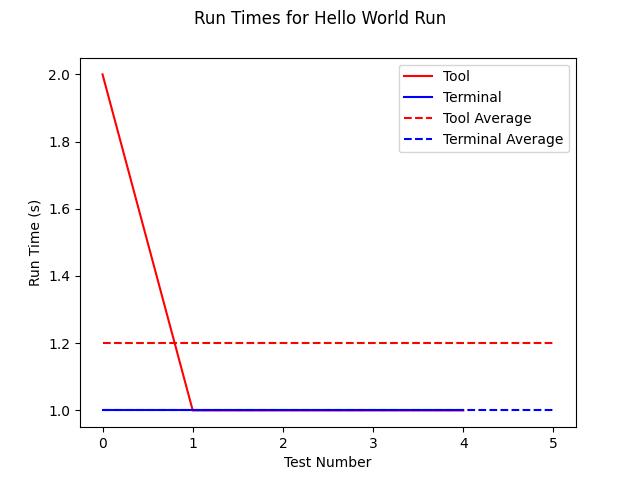
\includegraphics[width=3in]{images/evaluation/run5/hello-world}
  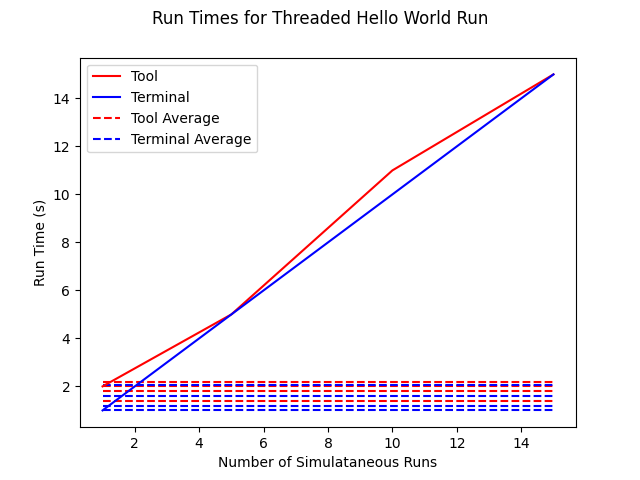
\includegraphics[width=3in]{images/evaluation/run5/thread-hello-world}
  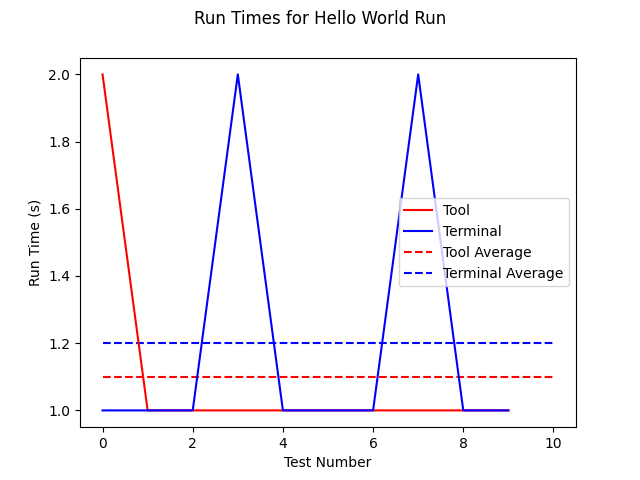
\includegraphics[width=3in]{images/evaluation/run6/hello-world}
  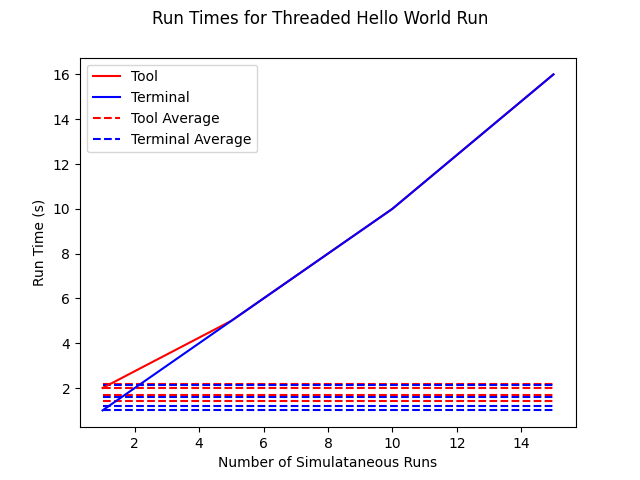
\includegraphics[width=3in]{images/evaluation/run6/thread-hello-world}
  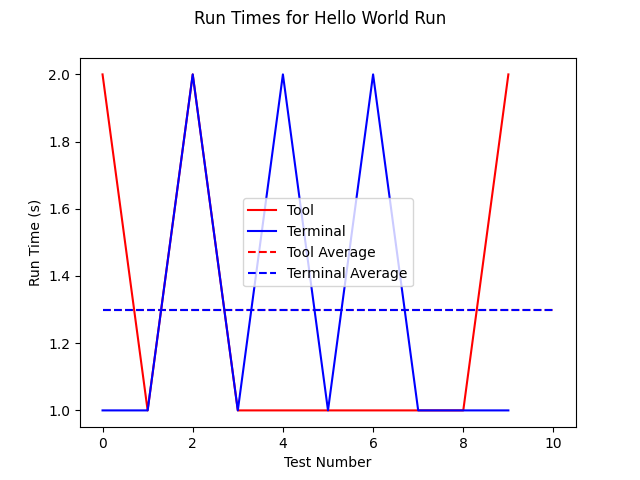
\includegraphics[width=3in]{images/evaluation/run7/hello-world}
  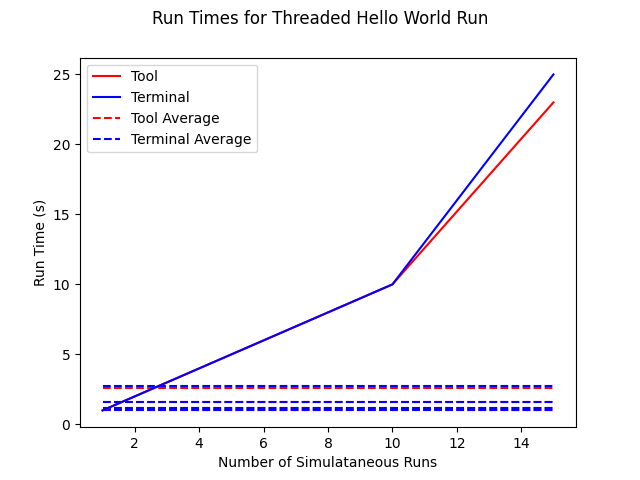
\includegraphics[width=3in]{images/evaluation/run7/thread-hello-world}
  \caption{Hello World Run Times}
  \label{img:helloWorld}
\end{figure}

\begin{figure}[h!]
  \centering
  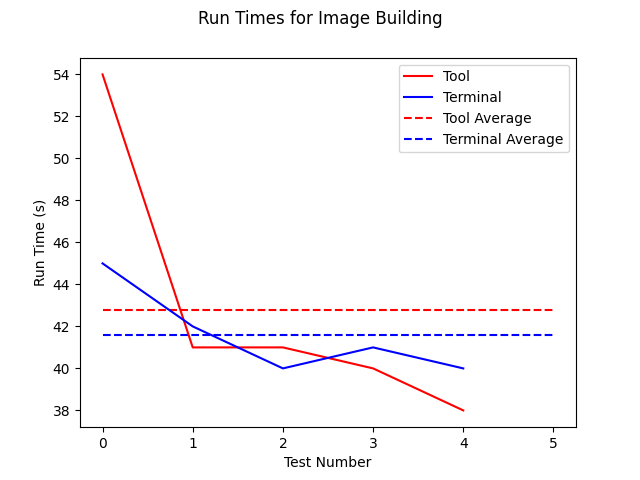
\includegraphics[width=3in]{images/evaluation/run5/image-build}
  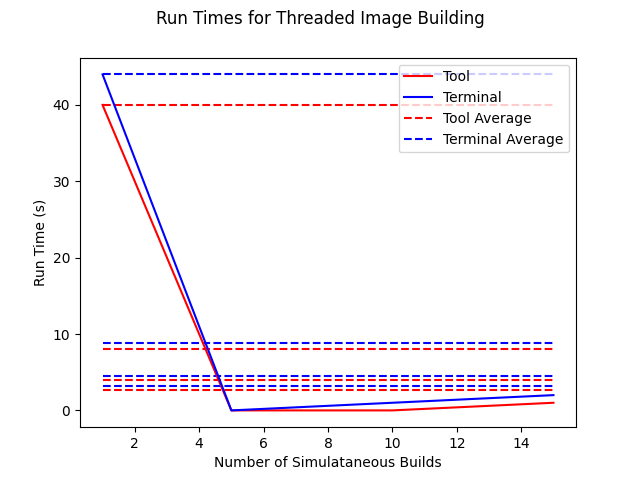
\includegraphics[width=3in]{images/evaluation/run5/thread-image-build}
  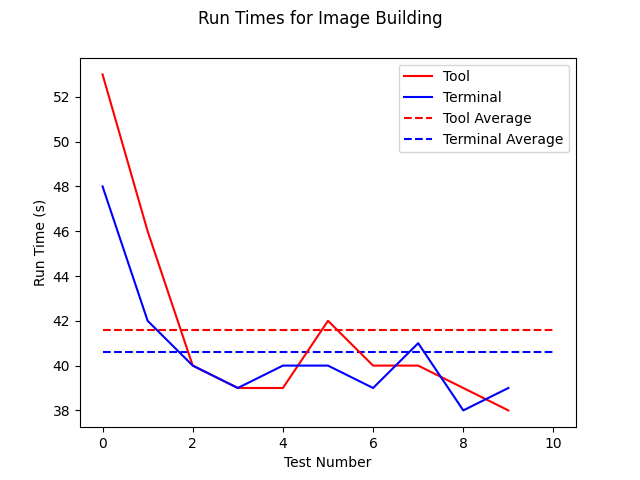
\includegraphics[width=3in]{images/evaluation/run6/image-build}
  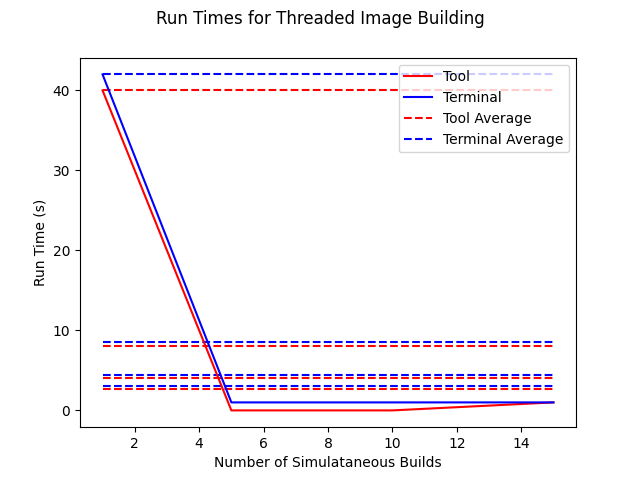
\includegraphics[width=3in]{images/evaluation/run6/thread-image-build}
  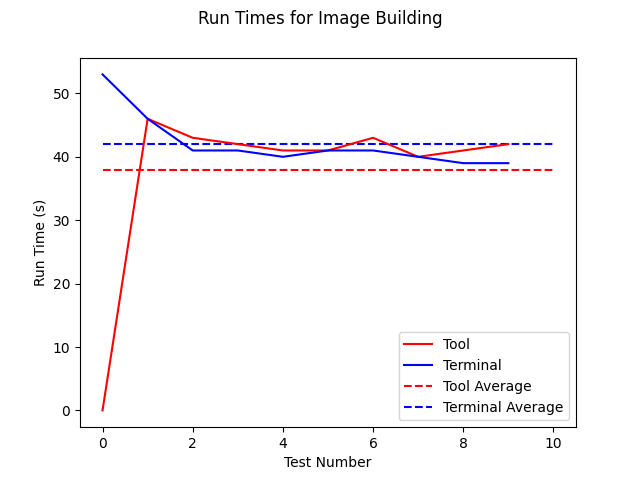
\includegraphics[width=3in]{images/evaluation/run7/image-build}
  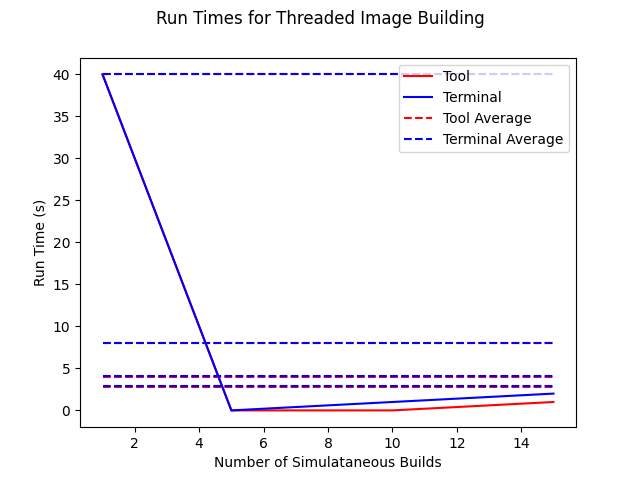
\includegraphics[width=3in]{images/evaluation/run7/thread-image-build}
  \caption{Image Build Run Times}
  \label{img:imageBuild}
\end{figure}

\begin{table}[h!]
\begin{tabular}{llllll}
Test Number & Test Type & \multicolumn{4}{l}{HELLO WORLD EVALUATION DATA}  \\
5           & Tool      & Times & 2, 1, 1, 1, 1                & Ave & 1.2 \\
            & Terminal  & Times & 1, 1, 1, 1, 1                & Ave & 1.0 \\
6           & Tool      & Times & 2, 1, 1, 1, 1, 1, 1, 1, 1, 1 & Ave & 1.1 \\
            & Terminal  & Times & 1, 1, 1, 2, 1, 1, 1, 2, 1, 1 & Ave & 1.2 \\
7           & Tool      & Times & 2, 1, 2, 1, 1, 1, 1, 1, 1, 2 & Ave & 1.3 \\
            & Terminal  & Times & 1, 1, 2, 1, 2, 1, 2, 1, 1, 1 & Ave & 1.3
\end{tabular}
\caption{Hello World Evaluation Data}
\label{tab:helloWorld}


\begin{tabular}{llllll}
Test Number  & Test Type  & \multicolumn{4}{l}{THREADED HELLO WORLD EVALUATION DATA}            \\
5            & Tool       & Times  & 2, 5, 11, 15  & Aves  & 2.0, 1.4, 1.8, 2.2                 \\
             & Terminal   & Times  & 1, 5, 10, 15  & Aves  & 1.0, 1.2, 1.6, 2.066666666666667   \\
6            & Tool       & Times  & 2, 5, 10, 16  & Aves  & 2.0, 1.4, 1.7, 2.2                 \\
             & Terminal   & Times  & 1, 5, 10, 16  & Aves  & 1.0, 1.2, 1.6, 2.1333333333333333  \\
7            & Tool       & Times  & 1, 5, 10, 23  & Aves  & 1.0, 1.2, 1.6, 2.6                 \\
             & Terminal   & Times  & 1, 5, 10, 25  & Aves  & 1.0, 1.2, 1.6, 2.7333333333333334  \\
\multicolumn{6}{l}{Note: Tests used the following number of threads for operations: 1, 5, 10, 15}
\end{tabular}
\caption{Threaded Hello World Evaluation Data}
\label{tab:threadHello}


\begin{tabular}{llllll}
Test Number & Test Type & \multicolumn{4}{l}{IMAGE BUILDING EVALUATION DATA}          \\
5           & Tool      & Times & 54, 41, 41, 40, 38                     & Ave & 42.8 \\
            & Terminal  & Times & 45, 42, 40, 41, 40                     & Ave & 41.6 \\
6           & Tool      & Times & 53, 46, 40, 39, 39, 42, 40, 40, 39, 38 & Ave & 41.6 \\
            & Terminal  & Times & 48, 42, 40, 39, 40, 40, 39, 41, 38, 39 & Ave & 40.6 \\
7           & Tool      & Times & 0, 46, 43, 42, 41, 41, 43, 40, 41, 42  & Ave & 37.9 \\
            & Terminal  & Times & 53, 46, 41, 41, 40, 41, 41, 40, 39, 39 & Ave & 42.1
\end{tabular}
\caption{Image Building Evaluation Data}
\label{tab:imageBuild}


\begin{tabular}{llllll}
Test Number  & Test Type  & \multicolumn{4}{l}{THREADED IMAGE BUILDING EVALUATION DATA}         \\
5            & Tool       & Times  & 40, 0, 0, 1  & Aves  & 40.0, 8.0, 4.0, 2.7333333333333334  \\
             & Terminal   & Times  & 44, 0, 1, 2  & Aves  & 44.0, 8.8, 4.5, 3.1333333333333333  \\
6            & Tool       & Times  & 40, 0, 0, 1  & Aves  & 40.0, 8.0, 4.0, 2.7333333333333334  \\
             & Terminal   & Times  & 42, 1, 1, 1  & Aves  & 42.0, 8.6, 4.4, 3.0                 \\
7            & Tool       & Times  & 40, 0, 0, 1  & Aves  & 40.0, 8.0, 4.0, 2.7333333333333334  \\
             & Terminal   & Times  & 40, 0, 1, 2  & Aves  & 40.0, 8.0, 4.1, 2.8666666666666667  \\
\multicolumn{6}{l}{Note: Tests used the following number of threads for operations: 1, 5, 10, 15}
\end{tabular}
\caption{Threaded Image Building Evaluation Data}
\label{tab:threadBuild}

\end{table}


\section{Threats to Validity}
\label{sec:threats}

There are several threats to the validity of both the tool, as well as the evaluation tests. The first threat comes from the evaluation itself, which is that there are many ways the data produced can be interpreted. This is an aspect that is inherent with any kind of evaluation and is present within this evaluation. However, I believe that the data, in this case, is rather straight forward to interpret.

The next possible threat to validity is the Threaded Image Building test, which as previously discussed, is a factor of how the tests were written and to fix would require other tests to be completely rewritten. However, despite these issues and admitting that they could pose a threat, I do not feel that they do. The tests show that it is possible with the tool to run multiple builds at the same time, however, there will never be a time for the same image to be built multiple times in parallel. So this test, while failing in one account, does succeed in illustrating the potential of the tool.

Looking directly at the tool several parts do not directly threaten its validity but do question how well the tool meets its goal. The first part that does this is the error handling, which is currently very basic and while it covers most issues does not handle some higher-level issues. The main case of this occurring is if the user (using the graphical interface) attempts to delete an image that doesn't exist, there is no indication that the image does not exist. These kinds of issues are being worked on and should be fixed by the time of the final release.

An additional threat that was discussed in a fair amount of detail back in section \ref{sec:eval} is the lack of evaluation of the Docker Installer. As previously discussed this is something I am hoping to figure out before the final version is due, but in the meantime, I do consider a threat to the validity of the tool. Not quite in the same vein as this is the threat posed by non-Linux operating systems, primarily Mac OS. This is an operating system that I do not have access to and as a result, will not be able to verify the compatibility of my tool. The installation commands which were loaded into the instruction set for Mac OS were taken directly from the Docker website, but with no way to ensure that they work with my tool, Mac OS exists as a threat to validity.

The final threat to the validity of my tool once again is on the evaluation suite itself. This is a suite that was written and designed by myself, which may mean there are areas of the tool which I should have evaluated that I have not. This could be for a variety of reasons, ranging from not believing it to be necessary to simply not knowing a feasible way to fully evaluate all of the work that has been done. This all being said, I believe that what I have evaluated are the core components of the tool which can be evaluated automatically and generate results that hold the lowest level of bias and the highest level of correctness as possible.

% How can the system break. How reliable is the tool?


%\numberedchapter{Conclusion}
\chapter{Discussion and Future Work}
\label{ch:conclusion}

% This is the conclusion. You might want to leave it unnumbered, as it is now. If you want to number it, treat it like any other chapter.
%
% This chapter usually contains the following items, although not
% necessarily in this order or sectioned this way in particular.

This chapter will provide a conclusion of the overall project. This conclusion will be drawn from what has been discussed in previous chapters and the summaries of the different components of the project which can be read below in the Summary of Results section \ref{sec:summary}. Also included in this chapter will be a discussion of what work will and could be done in the future. This section like the Summary of Results is split up into subsections for each of the three main components of the overall tool.

\break

\section{Summary of Results}
\label{sec:summary}
% A discussion of the significance of the results
% and a review of claims and contributions.

The overall goal of the tool which I developed was to streamline the process by which a user installs and interacts with components of Docker. To do this I developed a three-part software tool that can install Docker automatically, generate Dockerfiles, and has a straight forward user interface. A summary of the success of each of these components can be read in the following subsections of this chapter and have been broken up into their components.

\subsection{Results of Installer}
\label{sec:installerResults}

The Installer can successfully identify the operating system and version/distribution that is being run. This property works for each of the major Linux distributions that have installation steps listed on Docker's website. However, as discussed within the Threats to Validity \ref{sec:threats}, this portion is not verified to work with any other operating system. Unfortunately, this does not meet the initial goal of the Installer, which was to be able to work on each of the major operating systems. Despite not being verified, the instructions for these operating systems doe exist within the instructions folder of the tool and can be verified at a later date.

However, even if the full installer is not functional, it still illustrates how such a system could be developed. It can handle the installation of software on four (at least) different operating systems, all with different instructions. This is all handled by a single file within the tool, so it is not a complex system either. As such, making improvements upon this system would be very easy to, though that will be discussed more in the Future Work section \ref{sec:installerImprove}.

\subsection{Results of Generator}
\label{sec:generatorResults}

The Generator can be given the path to a folder anywhere on the host machine and then analyzes the contents of it for program files. This information is then passed along and used to determine what needs to be installed in the image. The image itself is based on Debian Bullseye which uses the Apt package manager and as a result utilizes Apt packages when installing the requirements for each language. The decision to use Debian as a base arose from my familiarity with Apt from using Ubuntu, so using Debian which used the same package manager as Ubuntu seemed like a logical choice. This process enables the Generator to correctly build images that can run a variety of different programs ranging from Python to C. This list of languages, which will be discuessed in the future work section \ref{sec:generatorImprove}, is currently limited and not overly complicated. However, having a system which can automatically look at a folder and create an image specific to its needs is a large contribution and not something that necessarily exists.


\subsection{Results of Interface}
\label{sec:interfaceResults}

The Interface is simple in design and offers access to the core functionalities of Docker. These functions include building, running, and deleting both Docker images and containers along with several other functions that a user may find helpful. All images and containers are listed at the top of the pages for the user to quickly and easily identify what image or container they would like to run. The functionalities for images and containers are split onto separate pages to allow for more streamlined use and to eliminate possible confusion between the two. The Interface is able to work on any device with a web browser since it utilizes Python Flask to create a web page that acts as the Interface. This allows for the Interface to have no kinds of platform specifity, if the device can run Python programs and has even the most basic web browser it can use the Interface. This all being said there are improvements that need to be made to the Interface which will be discussed in greater detail in the future work section \ref{sec:interfaceImprove}


\section{Future Work}
\label{sec:future}

As the tool is right now, it is unfinished. Some of the work that needs to be done, I will be doing after the initial draft of this full document is due. However, some improvements can be made which I simply will not have the time to do myself before the final code is due. Like above I have divided this section into subsections to properly talk about each component separately.

\subsection{Installer Improvments}
\label{sec:installerImprove}

Many improvements can be made to the Installer, the main one being verified support for both versions of Windows and Mac OS. Other than this there are several other improvements which can be made, which I hope to do in the future.

The main improvement I hope to make is to get a more concise installer. What I mean by this is to try and have less generalization between operating systems and have specialized processes that can ensure proper installation and testing of the installation. As it currently stands the method of verifying that Docker is properly installed is to simply run the hello-world image that Docker provides. However, this does not necessarily ensure that Docker is fully working. In the past, I have installed Docker myself, before I started developing the Installer, and was able to run the hello-world image. Unfortunately, for some reason, I was unable to run any other commands. I was able to fix the issue, but that process involved uninstalling and then reinstalling Docker and ensuring that my user was properly set up to use it.

\subsection{Generator Improvments}
\label{sec:generatorImprove}

The Generator, as it is right now, is very simple. This was a slightly conscious decision to present the user with fewer choices and make the process simpler. However, this lack of choice is slightly constraining and is something I would like to change in the future. The main aspect I would like to change would be to allow for a user to specify the Linux distribution they would like to use as a base for the image that would be generated from the Dockerfile. This is something which I believe would not be very hard to develop, but would require a fair amount of thought when it comes to structuring the lookup for packages for different programming languages.

Another improvement comes in the form of the contents of the Dockerfile. As it is right now each Dockerfile, for the most part, is the same with the only points of possible difference being between what gets installed and where the files get placed in the running image. While this provides a good learning platform for writing custom Dockerfiles, utilizing the tool for this customization is something that I would like to add. Like the above improvement this is something which complexity wise would be rather simple, but making the process simple and straight forward for a user would be rather complex.

The final improvement I would like to make to the Generator is to improve how it identifies what programming languages are within a folder. Currently, the Generator simply looks at the filetype extension, however, this method is not perfect and does not cover all possibilities for program files. There are several other methods of identifying programming languages and this process would likely take a large amount of inspiration from the methods in which Github's linguist can identify programming languages. Unfortunately, the linguist only works within repositories and can not be utilized directly for this project. The other issue with utilizing the linguist is that it is written primarily in Ruby, not Python which was used for this project. So I would have to develop a system that mirrors Github's linguist in Python, which would take some time to get it to work properly.

\subsection{Interface Improvments}
\label{sec:interfaceImprove}

There are a lot of improvements which can be made to the Interface. Right now it is very simple with only three main pages, the landing page, the Images page, the Containers page, in addition to a help page.

The first improvement is probably the largest and most time-consuming. This improvement is an overhaul to the Interface to make it more user friendly and aesthetically pleasing. While the Interface is currently not horrible, there is a lot of room for improvement to how information is presented. Some components do not look quite right with the current layout and some issues with aspects of the Interface not behaving perfectly when there is a large amount of information on the screen. There is also some improvement that can be made to the backend Flask components to streamline the entire web server and make running the Interface more efficient.

The next improvement is to get a working terminal window integrated directly into the Interface. This improvement is something that was being worked on for a time and would have utilized Xterm.js \cite{xterm} which is a TypeScript plugin for websites that can be used to host a terminal in a web page. However, due to a lack of knowledge in the area of TypeScript, I was unable to integrate it. This improvement would mainly be for consolidating all aspects of the tool into the Interface as all components still work properly when using the Interface.

The final improvement that can be made is to have more functionalities of Docker on the Interface. Currently, the functions are limited to the most basic and common operations like running an image. However, there are functions of Docker which may be helpful for users to have access to when their knownledge of Docker advances. This includes functions like creating Docker volumes and showing what containers are running and what port it is running on. These kinds of improvements would allow for the tool to help a user grow in respect to their knowledge of Docker functions, but come secondary to improvements to some of the core components listed above.

\section{Conclusion}
\label{sec:conclusion}

As the tool exists right now it fulfills much of what I sent out to accomplish. It can properly identify and install the correct version of Docker onto a computer. Currently, this is limited to the Linux versions of Docker, but as discussed in the Installer Improvements section \ref{sec:installerImprove} is something which I hope to expand upon in the future. The Generator successfully creates Dockerfiles based off of a given folder with program files stored within. There are improvements like those mentioned previously \ref{sec:generatorImprove} which I would like to make but overall it meets all of the goals I set for it when creating this project. The Interface allows the user to interact with Docker without having to know how to use every command that Docker has. This can allow for the time to execute any commands to be cut down in comparison to running commands through the terminal. This is is supported by the overall similar average run times when running identical commands between the tool and the Terminal. However, like the other two components of the tool, some improvements can be made as previously mentioned \ref{sec:interfaceImprove}. All of these improvements would serve to elevate the tool to a higher state which would only serve as improvements to an already helpful system.



%----------------------------------------------------------------------------------------
%	BIBLIOGRAPHY
%----------------------------------------------------------------------------------------

\addtocontents{toc}{\vspace{2em}} % Add a gap in the Contents, for aesthetics
\unnumberedchapter{Bibliography} % Title of the unnumbered chapter
\bibliography{preamble/bibliography} % The references information are stored in the file named "bibliography.bib"


\end{document}
